% Chapter 1
% Litterature Review

\chapter{Research Questions} % Main chapter title

\label{Chapter1} % For referencing the chapter elsewhere, use \ref{Chapter1} 
This submission is a continuous of the work presented in 300973 Engineering Thesis 1: Preliminary Investigations. In this report, we presented our research questions originated from the literature review. These questions are the motivation of our work and they also address research gaps, constraints and limitations. Then a summary that outlines our main contribution to these questions is provided.
%----------------------------------------------------------------------------------------

% Define some commands to keep the formatting separated from the content 
\newcommand{\keyword}[1]{\textbf{#1}}
\newcommand{\tabhead}[1]{\textbf{#1}}
\newcommand{\code}[1]{\texttt{#1}}
\newcommand{\file}[1]{\texttt{\bfseries#1}}
\newcommand{\option}[1]{\texttt{\itshape#1}}

\section{Aims and Objectives}
The aim of the thesis is to achieve three specific objectives and to test its associated hypotheses.


Our first objective is to develop a neural network architecture suitable for human action recognition (HAR) using spatial-temporal features.This aim comprises a broad set of design choices and requires multiple trade-off decisions to be made. The following are a selection of questions within this aim.
\begin{enumerate}
    \item What data storage should be employed to prevent data overflow? Is there a feedback or notification system inbuilt?
    \item What are the graphic processing units (GPU) requirements of the device? What is the smallest, most efficient processor for the task?
    \item Which architecture is able to concatenate vision based and memory based model? Is the network model able to identify people actions from a trimmed/untrimmed video?  
    \item What should be the acceptable training accuracy, and can we achieve it from the chosen network?
\end{enumerate}\\
Model type has a huge impact of HAR performance, and as stated by \cite{lockhart2014limitations}, the model type vary according to how the generated model is used and dictate the training and test set. They identify three basic model types: Impersonal models, Personal models and hybrid models. This aim includes the development of a custom neural network architecture used to analyze the actions based on two conditions: Time and appearance. The network is also estimating the accuracy against ground truth data.\\ 

Our second objective is develop a robust data pre-processing  method to address intra-class and inter-class variation in each action.
The aim involves developing a data pre-processing pipeline. This includes obtaining the right parameters for each video that can successfully extract frames that satisfy the neural network architecture. The following are questions associated to this aim.
\begin{enumerate}
    \item What type of data transfer should be implemented? How large/small the data transfer can be?  
    \item Which video trimming method can suit all the data to get the action of interest frames? What is the accepted number of frame for each video before processing? 
    \item Which feature is responsible of eliminating the intra-class variation where actions in video are similar?
    \end{enumerate}\\
A study by  \cite{nazir2017inter} showed the challenging task for HAR due to substantial amount of variation in video data. These variations include cluttered background, scale and viewpoint variation, occlusion etc. They proved that the performance of recognition decreases in complex environments. To accomplish this we build a system that takes input the trimmed video data and break each video to frame that conceivably contains action of interest. The system can be controlled by user-defined parameters using object-oriented programming (OOP) method on the Python programming language.\\

Our third objective is to fine tune the model to suit the data without changing the entire architecture.
The target is a scheme of trial and error attempts that demonstrate the best set of hyper-parameters. The following are questions motivated by this aim.
\begin{enumerate}
    \item Which stochastic optimization method need to be implemented to train the network? What the largest/smallest gradient step need to be taken every iteration.
    \item Which type of activation function can introduce non-linearity to the system? 
    \item Can Dropout layer fix  over-fitting and under-fitting? Is adding Dense layer help in generate better classification?
    \end{enumerate}\\
    
\cite{diba2018spatio} and \cite{liu2018attentive} demonstrate the importance of fine tuning a neural network model in beating the performance of recent methods. Fine tuning can also make the study more trustworthy and realistic.\\
    
To achieve these objectives, we developed a collection of parameters to try on the network. We trained the network every time with different parameters, and we witnessed the results. Based on these results, we concluded which values should be set as input to build a less bias classifier.

\section{Main Contributions}
To answer the research questions mentioned in Section 1.1, in this thesis we have developed a system that can contribute toward reducing the limitations in the HAR research field. Therefore, we proposed two different types of neural networks architecture and tested them on the popular KTH dataset \cite{schuldt2004recognizing}. We have also developed a data pre-processing pipeline that is responsible of receiving video frames and breaking them down to continuous sequences while also focusing on the mathematical complexity of the neural network model in term of number of parameters and number of layers. We presented an extensive evaluation of all the proposed approaches in this manuscript. We compared our techniques with each other and with state-of-the-art approaches. Moreover, we present a deep analysis of the results. Using these experiments, we try to find an answer to the question “When and which approach should we apply depending on videos and actions?”. This contribution is mainly presented in Chapter 2. Final results show that the best approach to deal with HAR is to use a sequence model concatenated with a spatial model instead of only a spatial model. We also understood and learned that in order to acheive high accuracy the model must have less parameters and more neural network layers. At the end, we were able to achieve an accuracy of 92.23\% for a sequence model and 64.76\% for a spatial model.
%----------------------------------------------------------------------------------------

\chapter{Research Methodology}\label{ThesisConventions}
This chapter is constructed as follows: The first part gives a comprehensive summary of the popular human action dataset (section 2.2), which is used as a backbone for the thesis. Next, we explain our data split and cross-validation pipeline. Then, we introduced and describe our proposed approaches: section 2.3 describe the first convolutional neural network (CNN) architecture, then section 2.4 describes the spatiotemporal stream architecture which combine CNN and an additional Long short term memory (LSTM) layer. Finally, the proposed methods are evaluated, tested and compared.

\section{Introduction}
We introduce a unified deep neural network structure consisting of two architecture. Both methods use the same mechanism for feature detection, class label encoding, and classification. But the main difference is that the second model uses Long short term memory layer that retains and skip sequence from each video. This gave us the opportunity to compare these learned features an further compare both of the models. we compared the performance of both method on the challenging and well studied KTH dataset introduced by \cite{schuldt2004recognizing}.

\section{KTH Dataset}
The KTH dataset introduced by \cite{laptev2004recognizing} consists of approximately 599 clips each of six distinct human activities (walking, jogging, running, boxing, hand waving and hand clapping) conducted by 25 different persons. Each actor performs an activity in four scenarios: outdoors, outdoors with scale variation, indoors and indoors with scale variation. All spatial dimension in each video are down-sampled to 160×120 and They are an average of 25 in length. KTH dataset considered
one of the challenging datasets due to the changes in scenes and scale variation. Refer to Figure ~\ref{fig:datasetset1KTH} for a visualization of KTH dataset. 

\begin{figure}[th]
\centering
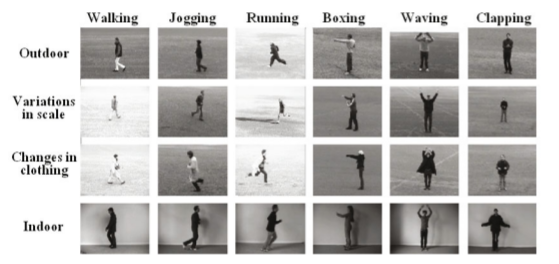
\includegraphics[width=0.85\columnwidth]{Chapters/photos/dt1.png}
\decoRule
\caption[A visualization of the KTH dataset \cite{schuldt2004recognizing}.]{A visualization of the KTH dataset \cite{schuldt2004recognizing}.}
\label{fig:datasetset1KTH}
\end{figure}\\

\section{Pre-processing of data}
For each experiment we split the data into three divisions: training split with examples used for training the classifier, validation split used to tune the parameters such as learning rate, regularization rate, optimization, etc. and test splits which contain data used for final assessment of the performance.\\

\begin{figure}[th]
\centering
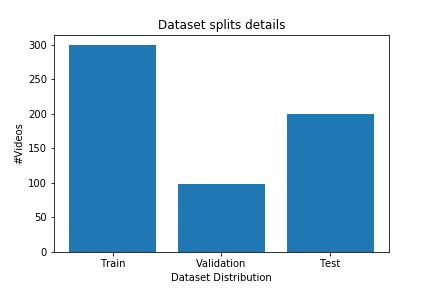
\includegraphics[width=0.83\columnwidth]{Chapters/photos/ds.png}
\decoRule
\caption[An illustration of the data splits method.]{An illustration of the data splits method.}
\label{fig:trainvalidtest}
\end{figure}\\

Technically, we create a program that take input the video directory. We then randomly dividing the whole data into 50\% for training equal to 300 videos, and 30\% for testing equal to 200 videos. Next, we take 25\% of the training data for validation. Finally, any remaining video is used for training the model. Refer to Figure ~\ref{fig:trainvalidtest} for visualization.

\subsection{Preprocessing Operation}
Video frame preprocessing is the term for operations on video frames or images at the lowest level of analysis. Generally, the aim of preprocessing operators
for HAR is to improve the image data by suppressing undesired degradations and simultaneously enhancing specific relevant features.\\

In this section, we describe and explain our robust preprocessing operators that are
important for enhancing video features and helpful in suppressing information that is not relevant in the video. This pipeline consists of 4 steps as follow.\\

\begin{figure}[ht]
\centering
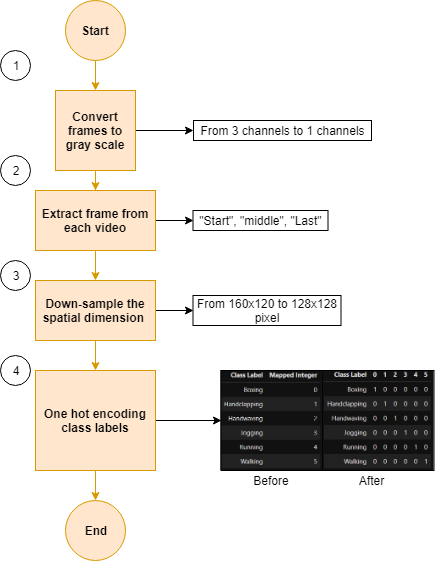
\includegraphics[width=0.5\columnwidth]{Chapters/photos/fc.png}
\decoRule
\caption[A flowchart show the steps followed to preprocess the video before feeding them to the network.]{A flowchart show the steps followed to preprocess the video before feeding them to the network.}
\label{fig:datapreprocessingpipeline}
\end{figure}\\

To simplify the computation power and complexity, we first take all frames in each video and convert them to grayscale. Although, KTH data are grayscale as described by the authors and motions in general are not defined by colors aspects, still a grayscale conversion is important to the system for final assessment and evaluation. Secondly, we program three options to extract video frames to facilitate the frame extraction, such as "start", "middle", "last". For our experiments, we know that action like "walking", "running" and "jogging" doesn't happen at the beginning of these videos which create lots of redundant and empty frames. This might affect the performance of our model. For that reason, we use the "middle" to extract the frames. We assume that each video has \textbf{M} frames in total, and the selected frames are defined by \textbf{N}. There are (\textbf{M} - \textbf{N}) frames. We would remove the first and last $\LARGE \frac{M-N}{2}$. Next, we downsample to spatial dimension from 160x120 to 128x128 pixel resolution, to ensure that all data have similar input size. Finally, we convert the input categorical labels into integers, then we apply One hot encoding on these integers labels, where the encoded labels (integers) are converted to binary variable that represent each categorical classes. Refer to Table ~\ref{tb:onehotencoding} and Table ~\ref{tb:onehotencoding2} for an illustration of One Hot Encoding and Figure ~\ref{fig:datapreprocessingpipeline} for visualization of the data pre-processing flowchart.

\begin{table}[ht]
\caption{How the class labels are mapped before one-hot encoding}
\centering
\begin{tabular}{|c|c|}
\hline
\textbf{Class Label} & \textbf{Mapped Integers} \\ \hline
Boxing               & 0                        \\ \hline
Handclapping         & 1                        \\ \hline
Handwaving           & 2                        \\ \hline
Walking              & 3                        \\ \hline
Jogging              & 4                        \\ \hline
Running              & 5                        \\ \hline
\end{tabular}

\label{tb:onehotencoding}
\end{table}
\begin{table}[ht]
\caption{How the class labels are mapped after one-hot encoding.}

\centering
\begin{tabular}{|c|c|c|c|c|c|c|}
\hline
\textbf{Class Label} & \textbf{0} & \textbf{1} & \textbf{2} & \textbf{3} & \textbf{4} & \textbf{5} \\ \hline
Boxing               & 1          & 0          & 0          & 0          & 0          & 0          \\ \hline
Handclapping         & 1          & 1          & 0          & 0          & 0          & 0          \\ \hline
Handwaving           & 2          & 0          & 1          & 0          & 0          & 0          \\ \hline
Walking              & 3          & 0          & 0          & 1          & 0          & 0          \\ \hline
Jogging              & 4          & 0          & 0          & 0          & 1          & 0          \\ \hline
Running              & 5          & 0          & 0          & 0          & 0          & 1          \\ \hline
\end{tabular}
\label{tb:onehotencoding2}
\end{table}


\section{Model Architecture 1: CNN}
In this section, we introduced our proposed CNN architecture, and we give a comprehensive explanation of our methodology. First, we briefly described the fundamental of a CNN model. Then we explain the reason behind the choice of activation function, regularization method, global average pooling (GAP) layer and its advantages toward the model parameters. Finally, we provide a visualization for the overall architecture.  

\subsection{What is a CNN model?}
CNN is a category of neural networks that recently have proven very effective in areas such as supervised classification and image recognition. CNNs have been successful in identifying the object at a microscopic scale empowering vision in medical images and nanotechnology applications. Convolutional networks were first introduced by \cite{lecun1989generalization}, as a special kind of network for processing data that has an understandable grid-like topology.\\

Convolution helps a machine learning system by leveraging three critical ideas, such as sparse interactions, equivariant representations and parameter sharing. Sparse interactions refer to sparse connectivity or sparse weights, and this is accomplished by making the kernel smaller than the inputs. For example, an input image might contain thousands of pixels, and the detection is performed on small meaningful features such as edges with kernels that occupy only tens or hundreds of pixels. This means that storing fewer parameters and operations, will both reduces the memory requirements of the model and improves its statistical efficiency. Parameter sharing refers to the usage of the same parameter for more than one function in a model. This means that the convolution operation learns a separate set of parameters for every location. This does not affect the run-time of forwarding propagation, but it does reduce the storage requirements of the model to $k$ parameters. As a result, convolution is then extremely efficient than dense matrix multiplication regarding memory requirements and statistical efficiency. Figure ~\ref{fig:la} graphically represents how parameter sharing works.
\begin{figure}[th]
\centering
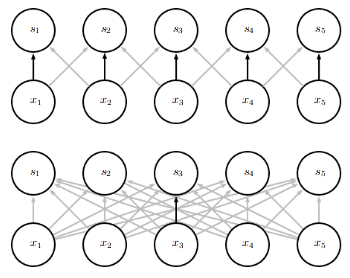
\includegraphics{Figures/ps}
\decoRule
\caption[The black arrow indicates the connections that use a particular parameter in two different model. \textit{(Top)} Black arrows indicate the usage of the centre of a three element kernel in a convolutional model. Due to parameter sharing, a single parameter is used at all input locations. \textit{(Bottom)} Black arrows indicate the usage of the central element of the weight matrix in a fully connected model. The model has no parameter sharing. As a result, the parameter is used only once \parencite{goodfellow2016deep}]{The black arrow indicates the connections that use a particular parameter in two different model. \textit{(Top)} Black arrows indicate the usage of the centre of a three element kernel in a convolutional model. Due to parameter sharing, a single parameter is used at all input locations. \textit{(Bottom)} Black arrows indicate the usage of the central element of the weight matrix in a fully connected model. The model has no parameter sharing. As a result, the parameter is used only once \parencite{goodfellow2016deep}}
\label{fig:la}
\end{figure}\\

As a result, sparse connectivity and parameter sharing can dramatically improve the efficiency of a linear function for detecting significant edges in an image. Figure ~\ref{fig:lala} shows both of these first two principles in action.\\

In convolution, the form of parameter sharing causes the layers to have a property called equivariance to translation. Generally, a function is equivariant means that if the input changes, the output changes in the same way. With images, convolution creates the 2D map of where certain features appear in the input, if the object is moved in the input, its representation will move the same amount in the output. For example, when performing image processing, it is useful to detect edges in the first layer of a convolutional layer.\\

In the image the same edges may appear more or less everywhere, for that reason, it is practical to share parameter across the entire image. However, this is not the case when processing images that are cropped to be centred on an individual face. That is because different features should be extracted at different locations. For example, the part of the network processing the top of the face needs to find eyebrows, while the part of the network processing the bottom of the face needs to look for a chin. Convolution is not equivariant to some other transformations, such as changes in the scale or rotation of an image, and other mechanisms are necessary for handling these kinds of transformations.\\

\begin{figure}[th]
\centering
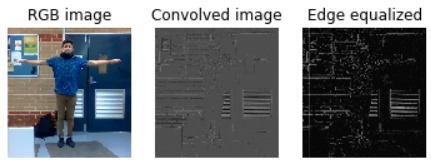
\includegraphics{Figures/edgedetection.png}
\decoRule
\caption[The image in the middle was formed by taking each pixel in the original image and subtracting the value of all vertically oriented edges in the input image. All images are 721 pixels tall. The input image is 681 pixels wide, while the output images are 680. This transformation can be described by a convolutional kernel containing two elements and requires 721*680*3=1,470,840 floating-point operations to compute using convolution. To describe the same transformation with a matrix multiplication would take 681*721*680*721, or over 240 billion entries in the matrix, making the convolution 240 billion times more efficient for representing this transformation]{The image in the middle was formed by taking each pixel in the original image and subtracting the value of all vertically oriented edges in the input image. All images are 721 pixels tall. The input image is 681 pixels wide, while the output images are 680. This transformation can be described by a convolutional kernel containing two elements and requires 721*680*3=1,470,840 floating-point operations to compute using convolution. To describe the same transformation with a matrix multiplication would take 681*721*680*721, or over 240 billion entries in the matrix, making the convolution 240 billion times more efficient for representing this transformation}
\label{fig:lala}
\end{figure}\\

A CNN model is made up of Layers. Every layer transforms an input 3D volume of activations to an output 3D volume with some differentiable function that may or may not have parameters as well as additional hyperparameters. There are distinct types of layers such as Convolutional layer, Pooling layer and a fully connected layer. Stacking these layers together will form a convolutional neural network architecture. In the following subsections, we describe each individual layers and the details for their hyperparmeters and their unique connectivities. Figure ~\ref{fig:standardCNN} presents a CNN model architecture with all its required layers and mathematical operations.
\begin{figure}[th]
\centering
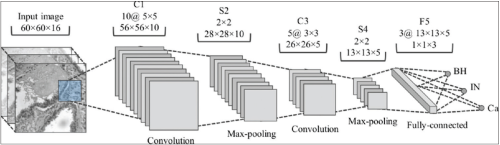
\includegraphics{Figures/cnn}
\decoRule
\caption[A visualization of a CNN architecture consisting of an input image of 60*60*16 followed by two convolutional layers and two max pooling layers and then followed by a fully connected layer \parencite{haj2017classifications}]{A visualization of a CNN architecture consisting of an input image of 60*60*16 followed by two convolutional layers and two max pooling layers and then followed by a fully connected layer \parencite{haj2017classifications}}
\label{fig:standardCNN}
\end{figure}\\

\subsection{Model Architecture}
This model is specifically designed to process RGB videos data. We choose to apply 3D CNN models inspired by popular the pretrained model AlexNet by \cite{krizhevsky2012imagenet}, due to its reputable performance on several types of data specially HAR related tasks. Since our videos are 3 dimensional, including time, we believe that 3D convolutional layers are more efficient due to their capabilities in learning spatial features.\\

Technically, our model consists of 5 convolutional groups, each of these groups has one or more convolutional layers, one max pooling layer and a LeakyReLU function, followed by a global average pooling (GAP), two fully connected layer, a dropout  layer and a  softmax layer to predict the final classification score of each class. Several decisions was made to found the best combination of layers. These decisions range from:
\begin{enumerate}
    \item Choosing the best sliding window filter for each convolutional layer and max pooling layer.
    \item Find the best combination of CNN layer that downsample the input frames to an even size before flatten these image's pixels to a 1D array.
    \item Find the best regularization method to reduce overfitting and vanishing gradient.
    \item Finding the right activation function to classify the spatial features.
    \item Finding the best optimization method that speed up the training time without affecting the model accuracy.
\end{enumerate}
The next section (sections 2.4.3-2.4.6) give a step by step explanation of these design decisions.
\begin{figure}[ht]
\centering
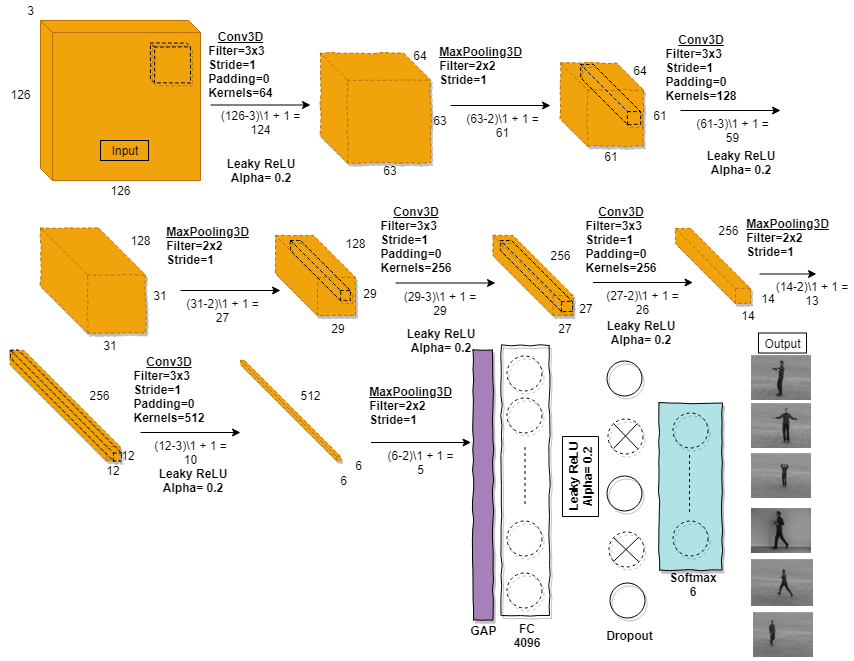
\includegraphics[width=0.85\columnwidth]{Figures/nn2.png}
\decoRule
\caption[A visualization of our proposed CNN architecture.]{A visualization of our proposed CNN architecture.}
\label{fig:la2}
\end{figure}

\subsection{Convolutional Layer}
\hspace{5mm} The convolutional layer is the core building block of a CNN model that does most of the heavy computation. In this section we will discuss the mathematical process of a convolutional layer.\\

Convolutional layer is a set of parameters consist of a set of learnable filters, where every filter is spatially along the width and the height, and also extend through the full depth of the input volume. The first filter has size of $3x3x1$ where $3$ is the pixels of the width and height of the image, and $1$ is its color channels, such as 1 grayscale and 3 for RGB. During the forward pass, we convolve each filter across the height and width of the input volume and calculate dot products between the entries of the filter and the input at any position. Since we are using 3D convolutional, a 3D activation map is produced everytime the filter slides over the input volume. The activation map give the responses of that filter at every spatial position. The network will then learn filters that activate when they spot some type of visual feature or pattern such as edge or blotch of some color on the first layer. On the other hand, each of these convolutional filters hold a stride and zero-padding. Stride is an instruction for the filter to shift at a certain unit at a time, in our case we set the stride to 1. Stride is normally set in a way so that the output volume is an integer and not a fraction. Zero-padding add zeros around the outside of the input volume so that the convolutions end up with the same number of outputs as inputs. For that reason, we set zero-padding to zero, to preserve as much as information about the original frame.\\
We calculate the size of the convolutional layer output tensor based on the this formula 

\begin{equation}
    W_{2}=\frac{W1-F+2P}{S} +1
\end{equation}

\hspace{5mm} Where \textbf{W2} is the size of the output image, \textbf{W1} is the size of the input image, \textbf{F} is the receptive field size of the Conv Layer neurons, \textbf{P} is the amount of zero padding used, and \textbf{S} is the stride.\\

\begin{figure}[ht]
\centering
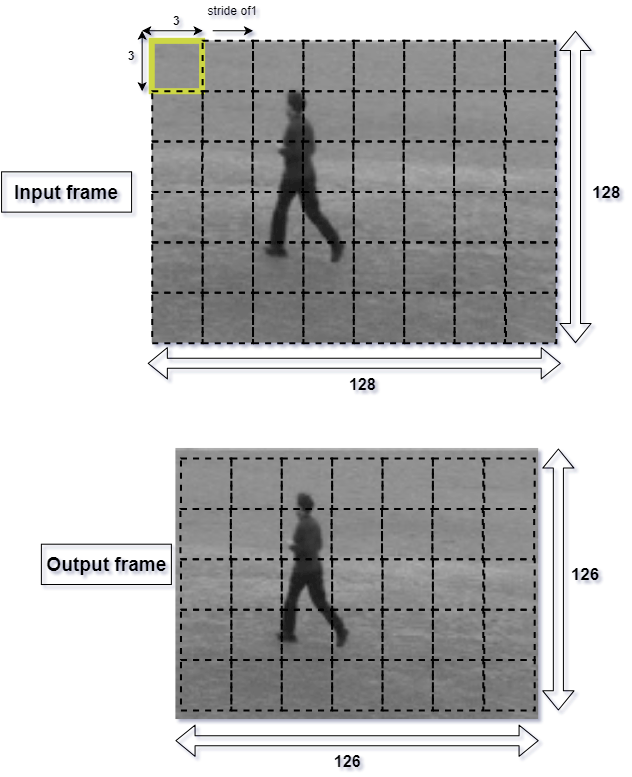
\includegraphics[width=0.8\columnwidth]{Figures/d1.png}
\decoRule
\caption[A visualization of the convolutional operation on one of the frame. The filter colored yellow has dimension of 3x3x1. We moved the convolutional 1 pixel at a time which is equal to stride of 1.]{A visualization of the convolutional operation on one of the frame. The filter colored yellow has dimension of 3x3x1. We moved the convolutional 1 pixel at a time which is equal to stride of 1. The output dimension are reduced from 128 to 126 pixels.}
\label{fig:la2la22}
\end{figure}

Having multiple filter in each convolutional layer produce a seperate 3D activation map for each filter. Stacking these activation maps along the depth dimension produce the output volume. Figure ~\ref{fig:la2la22} shows the convolutional operations in a 128x128 pixels frame.

\subsection{Max Pooling Layer}
\hspace{5mm} A pooling layer is another building block of a CNN and it is described as sample-based discretization process. This section describes the pooling operation of our convolutional network.\\

Convolutional networks may include local or global pooling layers which combine the outputs of neuron clusters at one layer into a single neuron in the next layer. It uses the maximum value from each of a cluster neuron at prior example, or it can also average this value. Its function is to progressively down-sample the spatial size of the representation to reduce the amount of parameters and computation in the network to learn and provides basic translation invariance to the internal representation.\\

Pooling operates independently in every depth slice of the input. The most common approach used in pooling is max pooling, also the one used in our CNN model. Max Pooling layer comes always after the convolutional operation by applying a max fitler to non overlapping subregions of the initial representation. It takes a filter of size 2x2 and stride of 1, and for each of the regions represented by the filter, it takes the maximum of that region and create a output matrix where each element is the max of the region in the original input. We calculate the size of the max pooling layer output tensor based on the formula below.

\begin{equation}
 W_{2}=\frac{W1-F}{S} +1
\end{equation}
This equation is obtained using the formula of the convolutional layer by making padding equal to zero. Refer for ~\ref{fig:maxpoolinglayervisualization} for maxpooling operation visualization.
\begin{figure}[ht]
\centering
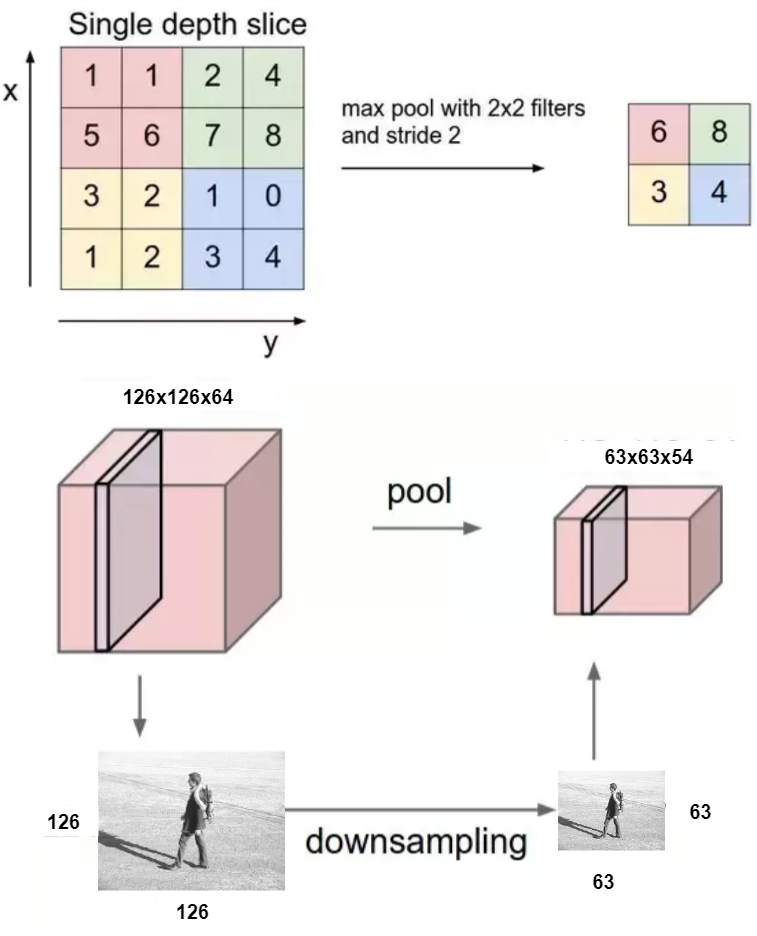
\includegraphics[width=0.6\columnwidth]{Figures/mp3.png}
\decoRule
\caption[A visualization of the max pooling operation on one of the frame. The input image has size of 126x126x64. We apply a max pooling with a filter of 2x2 with stride of 1. The output image become 63x63x64, where 64 is the kernel size.]{A visualization of the max pooling operation on one of the frame. The input image has size of 126x126x64. We apply a max pooling with a filter of 2x2 with stride of 1. The output image become 63x63x64, where 64 is the kernel size.}
\label{fig:maxpoolinglayervisualization}
\end{figure}

\subsection{Activation Function - LeakyReLU}

\begin{figure}[ht]
\centering
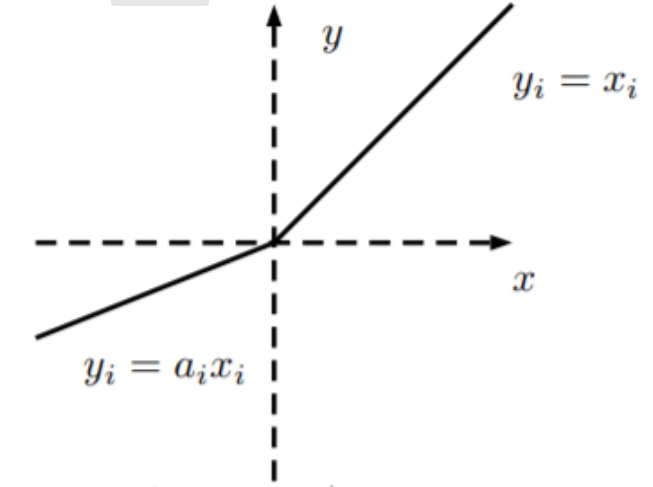
\includegraphics[width=0.6\columnwidth]{Figures/leakyrelu.PNG}
\decoRule
\caption[A visual representation of the Leaky ReLU activation function.]{A visual representation of the Leaky ReLU activation function.}
\label{fig:leakyreluactivationfunctions}
\end{figure}

Leaky ReLU was first introduced by \cite{xu2015empirical}. it is convention to apply a non linear layer or activation function immediately after every convolutional layer. The purpose of this layer is to introduce non linearity to a system that basically has just been computing linear operations during the convolutional layers. In the past, non linear functions like tanh and sigmoid were used, but researchers found out that leaky rectified linear unit (ReLU) work far better because the network is able to train a lot faster without making a significant difference to the accuracy. It also help to alleviate the vanishing gradient problem, which is the issue where the lower layers of the network train very slowly because the gradient decreases exponentially through the layers.\\

The reason behind choosing  this type of activation function is avoiding vanishing gradient and overfitting. Instead of the function being zero when x$\leq$ 0, a leaky ReLU will instead have a small negative slope (approximetly of 0.01 or more), as shown in Equation ~\ref{eq:la} and ~\ref{eq:la3} below.
\begin{equation}
\label{eq:la}
   \large  y_{i} = x_{i}, & x\geq 0
\end{equation}

\begin{equation}
\label{eq:la3}
   \frac{x_{i}}{a_{i}}, & x< 0
\end{equation}
\hspace{5mm} Here $y_{i}$, is the input of the non linear activation function of the \textit{i}th channels, and $a_{i}$ is a coefficient  controlling the slope of the negative part. The subscript \textit{i} in $a_{i}$ indicates that we allow the non linearity function to vary on different channels. Refer to Figure ~\ref{fig:leakyreluactivationfunctions} for Leaky ReLU activation function visualizayion.

\subsection{Regularization - Dropout}
Dropout is a stochastic regularization technique was first studied by \cite{srivastava2014dropout}. The term "dropout" refers to removing out units in the hidden layer of a network, with all its incoming and outgoing connections as shown in Figure ~\ref{fig:r}. In practice, the choice of dropping unit is random with a fixed probability $\large \rho$ independent of the other unit, where $\large \rho$ can be chosen using a validation set or can simply be set at 0.5. This makes their contribution to the activation temporally removed on the forward pass and any weight updates are not applied on the backward pass. These neurons become less sensitive to the weight update of the model. One of the advantages of using Dropout is generating better generalization and reduce over-fitting the training data.\\

In our experiment, we dropped approximately 20\% of
the hidden layers to make other neurons step in and handle the representation required to make predictions for the
missing neurons. This result in multiple independent internal representations being learned by the network after each
iteration.

\begin{figure}[ht]
\centering
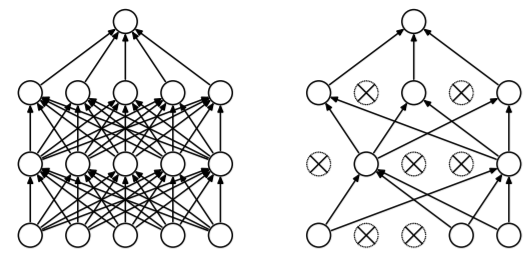
\includegraphics[width=0.6\columnwidth]{Figures/do}
\decoRule
\caption[\textbf{Left:} shows a standard neural network with 2 hidden layer. \textbf{Right:} shows the same network but with dropout applied to its hidden layers.]{\textbf{Left:} shows a standard neural network with 2 hidden layer. \textbf{Right:} shows the same network but with dropout applied to its hidden layers.}
\label{fig:r}
\end{figure}

\subsection{Model Parameters}
Generally, each layer has two kinds of parameters such as weights and biases. Hence, the sum of these two represents the model parameters. In practice, the number of parameters is proportional to the model complexity and model performance. On the other hand, having more parameters makes the model flexible and behave better with regularization and fine tuning.\\

In our architecture Figure ~\ref{fig:la2}, the input is an image of size 128*128*3. After Conv3D-1, the size of changes to 126x126x96 which is transformed to 63x63x96 after MaxPool3D-1. After Conv3D-2, the size changes to 61x61x128 and following MaxPool3D-2 it changes to 31x31x128. Conv3D-3 transforms it to a size of 29x29x256, then Conv3D-4 downsample this image to 27x27x256 and MaxPool3D-3 changes the size to 14x14x256, then Conv3D-5 reduce it to 12x12x512. Finally, GAP reduces the size to 6x6x512. This image feeds into FC-1 which transforms it into a vector of size 4096×1. The size remains unchanged through Dropout, and finally, we get the output of size 6×1 after Softmax layer. We calculate these two parameters according to following formulas.\\
\begin{itemize}
    \item \textbf{Number of Parameters of a Convolutional Layer}
    \begin{equation}
         W_{c} = O^{2} \ast N \ast F
    \end{equation}
\begin{equation}
     B_{c} = F
\end{equation}
\begin{equation}
     P_{c} = W_{c} + B_{c}
\end{equation}
Where:\\
\begin{itemize}
    \item \textbf{$W_{cf}$}: Number of weights of a fully connected Layer which is connected to a Convolutional Layer.
    \item \textbf{$B_{cf}$}: Number of biases of a fully connected Layer which is connected to a Convolutional Layer.
    \item \textbf{O}: Size (width) of the output image of the previous Convolutional Layer.
    \item \textbf{N}: Number of kernels in the previous Convolutional Layer.
    \item \textbf{F}: Number of neurons in the fully connected Layer.
    
\end{itemize}
    \item \textbf{Number of Parameters of a Max Pooling Layer}: There are no parameters associated with a Max Pooling layer. The pool size, stride, and padding are hyper-parameters.
    
    \item \textbf{Number of Parameters of a Fully Connected Layer}: There are two kinds of fully connected layers in a CNN. The first FC layer is connected to the last Conv Layer, while later FC layers are connected to other FC layers.
    \begin{equation}
 W_{cf} = O^{2} \ast N \ast F
\end{equation}
\begin{equation}
 B_{cf} = F
\end{equation}
\begin{equation}
 P_{cf} = W_{cf} + B_{cf}
\end{equation}

Where:\\
\begin{itemize}
    \item \textbf{$W_{cf}$}: Number of weights of a fully connected Layer.
    \item \textbf{$B_{cf}$}: Number of biases of a fully connected Layer.
    \item \textbf{O}: Size (width) of the output image.
    \item \textbf{N}: Number of kernels in the previous Convolutional Layer.
    \item \textbf{F}: Number of neurons in the fully connected Layer.
\end{itemize}
\end{itemize}
The total number of parameters in our model is the sum of all parameters in the 5 Conv Layers + 1 FC Layers + Dropout Layer. It 8,543,110 in total. Table ~\ref{tab:CNNmodelarchi} provides a summary of our CNN model parameters.


\begin{table}[ht]
\caption{Total number of parameters in our proposed neural network architecture.}
\centering
\begin{tabular}{|c|c|c|c|c|}
\hline
\textbf{Layer  name} & \textbf{Image} & \textbf{Weight} & \textbf{Biases} & \textbf{Params} \\ \hline
Input image & 128x128x1 & 0 & 0 & 0 \\ \hline
Conv3D & 126x126x64 & 576 & 64 & 1792 \\ \hline
MaxPool3D & 63x63x64 & 0 & 0 & 0 \\ \hline
Conv3D & 61x61x128 & 1152 & 128 & 221312 \\ \hline
MaxPool3D & 31x31x128 & 0 & 0 & 0 \\ \hline
Conv3D & 29x29x256 & 2304 & 256 & 884,992 \\ \hline
Conv3D & 27x27x256 & 2304 & 256 & 1,769,728 \\ \hline
MaxPool3D & 14x14x256 & 0 & 0 & 0 \\ \hline
Conv3D & 12x12x512 & 0 & 0 & 0 \\ \hline
MaxPooling3D & 6x6x512 & 0 & 0 & 0 \\ \hline
GAP & 512x1 & 0 & 512 & 0 \\ \hline
Dense & 4,096x1 & 4,096,000 & 4,096 & 2,101,248 \\ \hline
Dropout & 4,096x1 & 0 & 4,096 & 0 \\ \hline
Output & 6 & 0 & 0 & 24582 \\ \hline
Total Params & \multicolumn{4}{c|}{8,543,110} \\ \hline
\end{tabular}
\label{tab:CNNmodelarchi}
\end{table}\hfill


\subsection{Global Average Pooling}
\hspace{5mm} Conventional CNN perform convolutional in the lower layers of the network. As a results, \cite{lin2013network} proposed a new strategy called global average pooling, as a replacement to the traditional fully connected layer. GAP layer generate one feature map for each corresponding category of the classification. That's said, instead of adding fully connected layers on top of the feature maps, we take the average of each feature map, and the resulting vector is fed directly into the softmax layer for final prediction. One advantage of GAP layers is that it is more native to the convolution structure by enforcing correspondences between
feature maps and categories. Thus the feature maps can be easily interpreted as categories confidence
maps. Another advantage is that there is no parameter to optimize in the global average pooling
thus over-fitting is avoided at this layer. Furthermore, global average pooling sums out the spatial
information, thus it is more robust to spatial translations of the input.\\

In our experiment, the number of parameters increases in each layer. An architecture like this is more likely to over-fit during training. For that reason, we used GAP layer to reduce our model parameters before it reaches fully connected layers. As an example, the number of parameters in our model are reduced from 3,539,456 to 2,101,248 after GAP is applied Table ~\ref{tab:CNNmodelarchi}. Figure ~\ref{fig:gap} shows tensor with dimensions h*w*d is reduced in size to have dimensions 1*1*d. GAP layers reduce each h×w feature map to a single number by simply taking the average of all h*w values.

\begin{figure}[ht]
\centering
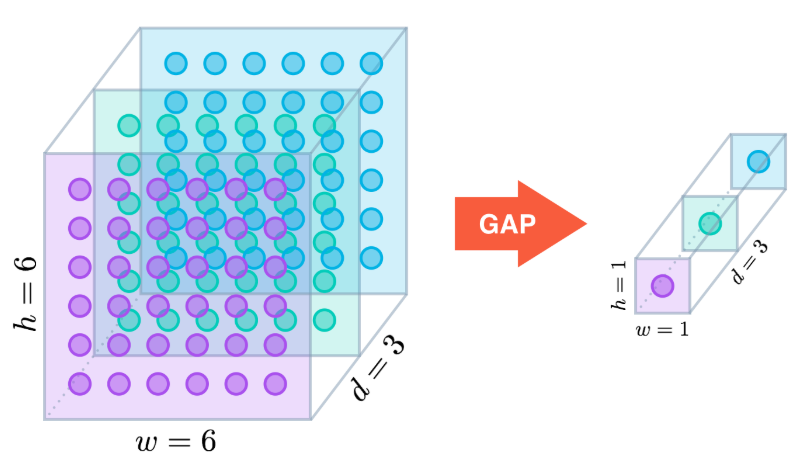
\includegraphics[width=0.6\columnwidth]{Figures/gap}
\decoRule
\caption[An example of a GAP applied on a 3D image \cite{lin2013network}.]{An example of a GAP applied on a 3D image \cite{lin2013network}.}
\label{fig:gap}
\end{figure}

%----------------------------------------------------------------------------------------


\section{Model Architecture 2: CNN-LSTM}
In this section, we introduce Recurrent neural network (RNN) architecture, and we give a comprehensive explanation of our methodology using CNN and RNN in one model. We first, describe briefly the fundamental of a RNN model, then we explain the reason behind the choice of our activation function, memory layer, wrapping the entire architecture with Time Distributed layer and the advantage of using batch normalization to speed up the training. Finally, we provide a visualization for the overall architecture.

\subsection{What is a RNN model?}

RNN are a family of neural network designed to recognize patterns in sequences of data, such as text, genomes and handwriting etc. These algorithms take time and sequence into account, they have a temporal dimension.
RNN was first introduced by \cite{rumelhart1986learning}, to be one of the most powerful and useful type of neural network, alongside the attention mechanism and memory networks. RNNs are applicable even to images, which can be decomposed into a series of patches and treated as a sequence.
Since recurrent networks possess a certain type of memory, and memory is also part of the human condition, we’ll make repeated analogies to memory in the brain.\\

RNN helps a machine learning system by leveraging one of the early ideas found in statistical model of the 1980s such as sharing parameters across different parts of a model. Parameter sharing makes it possible to extend and apply the model to examples of different forms and lengths and generalize across them. Such sharing is particularly important when a specific piece of information can occur at multiple positions within the sequence. Recurrent networks share parameters in a different way. Each member of the output is a function of the previous members of the output. Each member of the output is produced using the same update rule applied to the previous outputs.This recurrent formulation results in the sharing of parameters through a very deep computational graph.\\

While CNNs are effective at learning spatial features in single independent frames, a recurrent layer excels at integrating temporal context. \cite{tripathi2016context} defined a neural network architecture where the frame-by-frame object predictions of a pre-trained convolutional neural network where used as inputs to a recurrent layer. A similar approach is taken in these experiments, with the exception that the convolutional network is fine-tuned jointly with the training of the recurrent layer. The communication between the CNN and the RNN is learned concurrently with the optimization and is not limited to passing actual object class predictions. The RNN outputs the final predictions for each frame while taking previous frames into account using memory layer. Another example of CNN-RNN model, is the capability of predicting objects’ velocity vectors in the image plane. By allowing detections from previous frames to flow to the current frame via recurrent connections in the RNN layers, the network can keep track of moving objects across time and give estimates for the velocity.\\

The recurrent neural network is represented as shown in Figure ~\ref{fig:gap1}, and also shows the different types of RNN architecture in Figure ~\ref{fig:RNNmanytoonoetypes}. Each node at a time step takes an input from the previous node and this can be represented using a feedback loop. We can unfurl this feedback loop and represent it as shown in the figure below. At each time step, we take an input $x_{i}$ and $a_{i-1}$ (output of the previous node) and perform computation on it and produce an output $h_{i}$. This output is taken and given to the next node. This process continues until all the time steps are evaluated. In the following subsections, we describe each important layer that make our network unique and different from the previous architecture and the details for their hyper-parmeters and their unique connectivities.

\begin{figure}[ht]
\centering
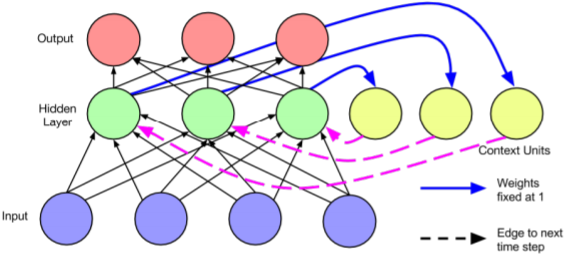
\includegraphics[width=0.60\columnwidth]{Figures/rnn}
\decoRule
\caption[An example of a recurrent neural network as described by \cite{elman1990finding}. Hidden
units are connected to context units, which feed back into the hidden units at
the next time step \citep{lipton2015critical}.]{An example of a recurrent neural network as described by \cite{elman1990finding}. Hidden
units are connected to context units, which feed back into the hidden units at
the next time step \citep{lipton2015critical}.}
\label{fig:gap1}
\end{figure}


\begin{figure}[ht]
\centering
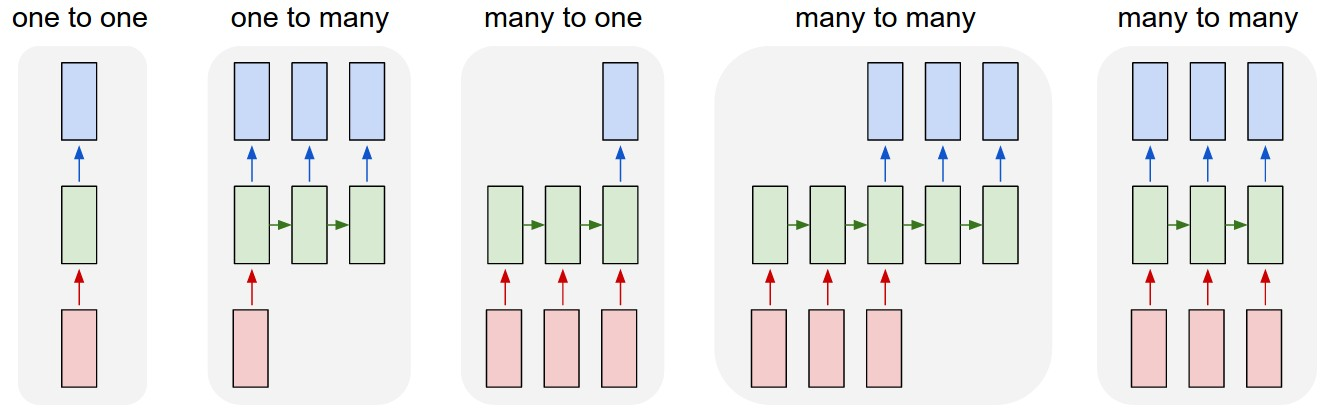
\includegraphics[width=0.8\columnwidth]{Figures/rn1}
\decoRule
\caption[A visualization of the most used RNN architectures. Red rectangles
correspond to inputs, Blue rectangles to outputs and green rectangles to the entire hidden state of the neural network. \textbf{One to one} Represents a conventional  feedforward networks. \textbf{One to many} Text and video classification are tasks in which a sequence is mapped to one fixed length vector. \textbf{Many to one}
Image captioning presents the converse case, where the input image is a single
non-sequential data point. \textbf{Many to many} This architecture has been used for natural language translation, a sequence-to-sequence task in which the two sequences may
have varying and different lengths. \textbf{Many to many} This architecture has been used to learn
a generative model for text, predicting at each step the following character \citep{lipton2015critical}.]{A visualization of the most used RNN architectures. Red rectangles
correspond to inputs, Blue rectangles to outputs and green rectangles to the entire hidden state of the neural network. \textbf{One to one} Represents a conventional  feedforward networks. \textbf{One to many} Text and video classification are tasks in which a sequence is mapped to one fixed length vector. \textbf{Many to one}
Image captioning presents the converse case, where the input image is a single
non-sequential data point. \textbf{Many to many} This architecture has been used for natural language translation, a sequence-to-sequence task in which the two sequences may
have varying and different lengths. \textbf{Many to many} This architecture has been used to learn
a generative model for text, predicting at each step the following character \citep{lipton2015critical}.}
\label{fig:RNNmanytoonoetypes}
\end{figure}

\subsection{Model Architecture}
This model architecture in Figure ~\ref{fig:lstmcnn} is an improvement of the previous model Figure ~\ref{fig:la2}. It consists of two phases: CNN and RNN-LSTM. Because our dataset consists of sequence of videos, a CNN with memory layers are used to process these sequences and learn spatial and temporal features from the videos.\\

The CNN model consists of one convolutional layers with 3x3 filter and a stride of 1, followed by a batch normalizationl layer for regularization, then using a ReLU as activation function, and max pooling layer with 2x2 filer and stride of 1, and adding Dropout as a second regularize with 0.25 dropping rate. These 4 layers are being repeated 3 times to downsample the image. After that, we add two fully dense (fully connected) layer each with 256 and 128 neurons respectively. For the second phase of this network, we build two networks of LSTM layers that take the CNN vector as input. This LSTM layers consists of a forget layer that remember the sequence of each frame and apply a tanh as activation function. Next, we know that the first layer is forward sequence while the second layer is a backward sequence. As a results, we concatenare these two layers, and apply a softmax layer that hold the action classes of the dataset. 
\begin{figure}[ht]
\centering
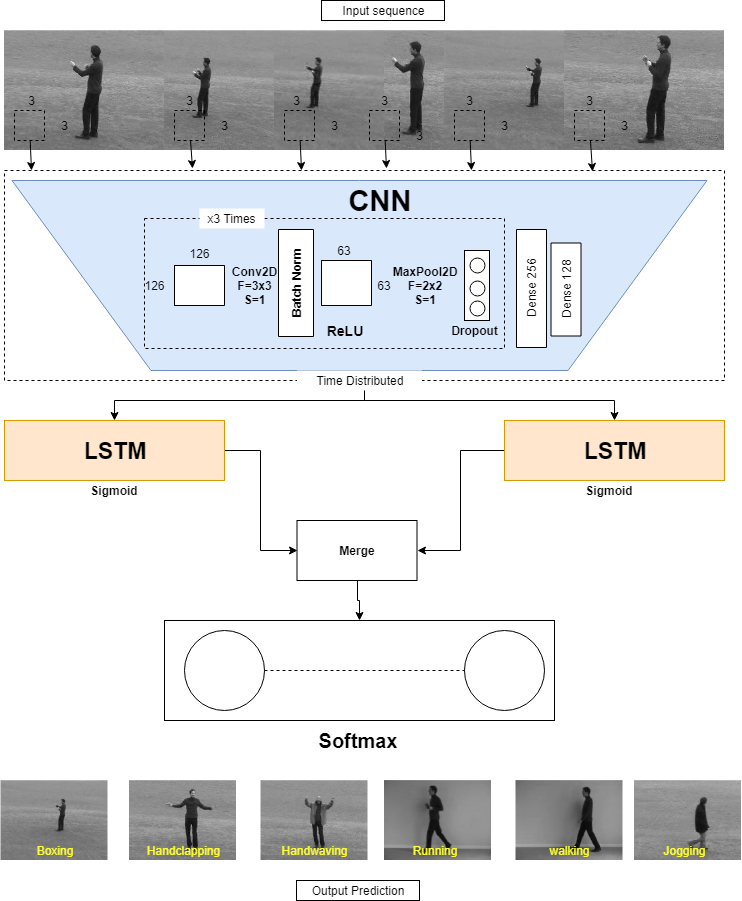
\includegraphics[width=0.75\columnwidth]{Figures/cnnlstm.png}
\decoRule
\caption[A visualization of our proposed CNN-LSTM model.]{A visualization of our proposed CNN-LSTM model.}
\label{fig:lstmcnn}
\end{figure}


\subsection{Long Short Term Memory}
\cite{hochreiter1997long} introduced the LSTM model, an extension of RNN, which stands for Long short term memory, primarily in order to overcome the problem of vanishing gradients and long-term dependency problem by explicitly learning when to modify the hidden state via gates.\\

Simple recurrent neural networks have long-term memory in the form of weights.
The weights change slowly during training, encoding general knowledge about
the data. They also have short-term memory in the form of ephemeral activation's, which pass from each node to successive nodes. The LSTM model
introduces an intermediate type of storage via the memory cell. A memory cell
is a composite unit, built from simpler nodes in a specific connectivity pattern,
with the novel inclusion of multiplicative nodes, represented by the
letter $\prod$ like in Figure ~\ref{fig:lstm}.\\

There are one input node, internal state and three gates: forget gate, input gate and output gate, each of which acts as a one layer neural network on its own.
\begin{itemize}
    \item \textbf{Input node}\\
    Takes activations in the standard way from the input layer at the current time step and along recurrent edges from the hidden layer at the previous time step. The output of each gate is limited to [0, 1] via a sigmoid activation and all gates observe both the previous hidden state and the current LSTM layer input.
    
\item \textbf{Input gate}\\
Controls when to use information present in the input. Its value is used to multiply the value of another node. It is a gate in the sense that if its value is zero, then flow from the other node is cut off. If the value of the gate is one, all
flow is passed through. The value of the input gate $i_{i}$ multiplies the value
of the input node

\item \textbf{Internal state}\\
The internal state $s_{c}$ has a self-connected recurrent edge
with fixed unit weight. Because this edge spans adjacent time steps with
constant weight, error can flow across time steps without vanishing or exploding. This edge is often called the constant error. In vector
notation, the update for the internal state is presented in Equation \ref{equation2.11}:
\begin{equation}\label{equation2.11}
     s^{(t)}=g^{(t)}\odot i^{(t)}+ s^{(t-1)}
\end{equation}

\item \textbf{Forget gate}\\
Outputs a multiplier vector for the hidden state, where zero output causes the hidden state to be discarded and one to be kept. With forget gates and according to \cite{gers1999learning}, the equation to calculate the internal state
on the forward pass is 
\begin{equation}
     s^{(t)}=g^{(t)}\odot i^{(t)}+f^{(t)}\odot s^{(t-1)}
\end{equation}
Where $s^{(t)}$ denotes internal state, $\odot$ denotes element-wise multiplication, \textbf{t} denotes the time state, \textbf{g} denotes current input for the sigmoid function, \textbf{i} and \textbf{f} denote the input gate.
\item \textbf{Output gate}
Controls how the hidden state influences the network output.
\end{itemize}

\begin{figure}[ht]
\centering
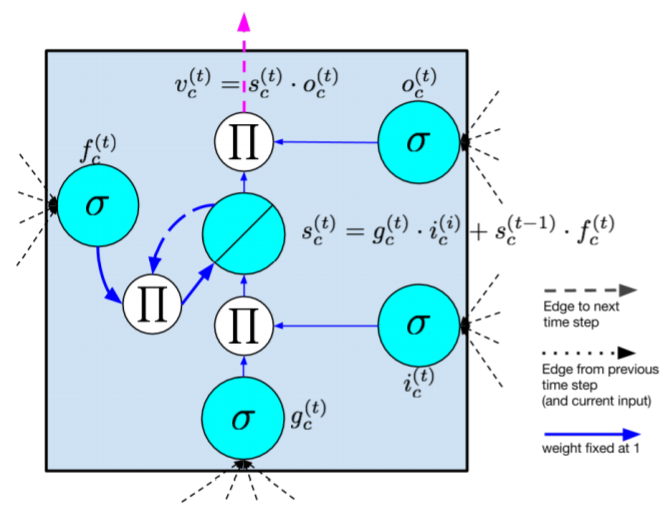
\includegraphics[width=0.80\columnwidth]{Figures/lstm}
\decoRule
\caption[An example of LSTM model as suggested by \cite{gers1999learning}.]{An example of LSTM model as suggested by \cite{gers1999learning}.}
\label{fig:lstm}
\end{figure}

All gates are learned simultaneously with the neural network, as all the
internal operations of the layer are differentiable and their effect to the final
loss function can be inferred. It can be said that during optimization the
LSTM learns which features of the input are worth keeping in the hidden
state and which features of the hidden state are not useful for prediction and
can be discarded.
By explicitly modifying the hidden state via learnable gates, the LSTM
sidesteps the vanishing gradients problem in simpler RNNs where long term
dependencies are easily lost after repeated transformations through a hidden
layer. In LSTM, the hidden state is modified only via the gates and it is very
easy for the state to flow through multiple time steps unchanged.\\

In our architecture and as shown in ~\ref{fig:lstmcnn}, there are two layers of LSTM. Both LSTMs layers are connected in parallel and take the CNN model as input and they are being concatenated afterwards. They are differentiated in that the left LSTM takes a 1x128 input dimension and output this dimension to 1x256. It has one forget bias unit, that return a sequence with a Tanh activation function and an inner Sigmoid activation function. While right LSTM layer preserves the same specification, but it reverses the given sequence. 

\subsection{Activation Function - ReLU}

\begin{figure}[ht]
\centering
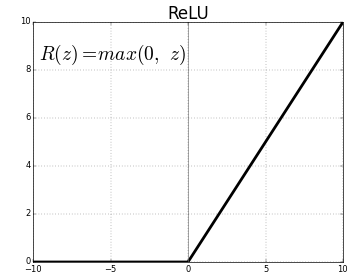
\includegraphics[width=0.80\columnwidth]{Figures/relu.png}
\decoRule
\caption[A visual representation of the ReLU activation function \cite{nair2010rectified}.]{A visual representation of the ReLU activation function \cite{nair2010rectified}.}
\label{fig:relu1}
\end{figure}
Rectified linear unit was first introduced by \cite{nair2010rectified}, as a function that have a non linear property without affecting the receptive field on the network. It's advantage consists in speeding up training and avoiding vanishing gradient, its equation can be written as below.\\

\begin{equation}\label{eq:1}
    \ y_{i} =x_{i}, & x\geq 0
\end{equation}

\begin{equation}\label{eq:2}
    0, & x \leq 0
\end{equation}

In practice, ReLU returns 0 Equation ~\ref{eq:2} if it receives any negative input, but for any positive value x it returns that value back Equation ~\ref{eq:1}. It can be written as $\large R_{(z)}=max(0,z)$, as shown in Figure ~\ref{fig:relu1} above.\\

ReLU serve two primary purposes in our model:
\begin{itemize}
    \item Help the model account for interaction effects.
    \item Help the model account for non-linear effects.
\end{itemize}
\textbf{Interactions:} The weight from the model creates interactions during training, and adding more layers and more nodes, the potential complexity of interactions only increases, in this case ReLU captures this interaction and helps in taking only positive value to help the classification model produce high accuracy for each action labels.
\textbf{Non-linearity:} In our model, we include bias for each node, which is a constant number that is determined during model training. This bias term allow us to move where the slope changes. As a result, each node change slope at different values for our output.\\

Overall, this activation have more flexibility to produce non-linearity functions and account for interactions to give better predictions, and the performance increase as the model complexity increase.

\subsection{Time Distributed Layer}
We using a CNN-RNN, that's mean, we are dealing with a sequence classification problem. It is essential to make the dense nodes of the layer identical and share the same weights and biases, using a time distributed layer applied fully connected dense on each time step and get output separately by time steps.\\

Technically, Time distributed layer applies same as a dense layer or a fully connected layer to every time step of a 3D tensor. This wrapper applies a layer to every temporal slice of an input. In our case the input, is a 3D tensor, and the dimension of index one is considered to be the temporal dimension. We used time distributed layer to all our Con3D and Max Pooling3D layers, to add an additional temporal layer. This creates a spatial vector from each frame, and associate them with an additional temporal vector for every sequence. The network then remembers each frames according to its spatial feature and appearance.

\subsection{Batch Normalization}
The distribution of each layer's inputs change during training, as the parameters of the previous layers change. This slows down the training by requiring lower learning rates and careful parameter initialization, and makes it notoriously hard to train models with saturating non-linearities. We refer to this phenomenon as internal covariate shift as suggested by \cite{ioffe2015batch}. Making normalization a part of the model architecture and performing the normalization for each training mini-batch. Batch Normalization allows us to use much higher learning rates and be less careful about initialization. It also acts as a regularizer, in some cases eliminating the need for Dropout, however, we still used dropout, as a second regularization layer. Using batch normalization, allow us to beats the original model by a significant margin.\\

We seek to reduce the internal covariate shift. By fixing the distribution of the layer inputs x as the training progresses, we expect to improve the training speed. \cite{lecun2012efficient} said that the network training converges faster if its inputs are whitened, for example, linearly transformed to have zero means and unit variances, and de-correlated. By whitening the inputs to each layer, we would take a step towards achieving the fixed distributions of inputs that would remove the ill effects of the
internal covariate shift.\\

The normalization can then be written as a transformation like in Equation \ref{normalizationfortranf} below:
\begin{equation}\label{normalizationfortranf}
     \widehat{x}=Norm(x,X)
\end{equation}
where \textbf{x} is the input layer, treated as a vector, and \textbf{X} is the set of these inputs over the training data. It depends not only on the given training example x but on all examples X, each of which depends on $\Theta$ if
x is generated by another layer. On the other hand, for back-propagation, we compute the Jacobians.

\begin{equation}\label{derivative1}
     \frac{\delta Norm(x,X)}{\delta x}
\end{equation}

\begin{equation}\label{derivative2}
    \frac{\delta Norm(x,X)}{\delta X}
\end{equation}
Where $\delta$ is derivation symbol for both Equation \ref{derivative1} and Equation \ref{derivative2}. 
The  aim is to preserve the information in the network, by
normalizing the activations in a training example relative
to the statistics of the entire training data.\\

In our experiment, batch normalization, is a part of our neural network structure, approximates this process by standardizing the activations using a statistical estimate of the mean $\widehat{E}(x)$, and standard deviation $\widehat{Var}(x)$  for each mini batch training. The below formula represents the batch normalization.
\begin{equation}
        BN\left ( x;\gamma ,\beta \right )=\gamma \frac{x-\widehat{E}(x)}{\sqrt{\widehat{Var}(x)+\epsilon }} +\beta
\end{equation}
Where $\gamma$ and $\beta$ are scale and shift parameters for the activation $x$. An identity transformation is then presented for each activation. The $\epsilon$ is a constant added as a regularization parameter for numerical stability. The division is performed element wise. $\gamma$ and $\beta$ are learned during training and fixed during inference.\\

To take full advantage of batch normalization technique, we change the network and its training parameters, such as, increasing learning rate, removing dropout, accelerate the learning rate decay, remove local response normalization, and shuffle the training example more thoroughly.

\section{Training and Testing}
Neural networks are very complex models and obtaining good results can be
difficult. This chapter describes many practical methods used to train and test our proposed neural network architecture described in Figure ~\ref{fig:la2} and Figure ~\ref{fig:lstmcnn}.

\subsection{Initialization}

Proper initialization can have a
great impact on both the speed of the training and the evaluation accuracy
of the model. Poorly initialized models can even fail to converge. Before training can begin, the initial values for the parameters of the network,
the weights and biases are selected. 
Initializing all network parameters to zero, each neuron would
receive the same learning signal from the optimizer that is minimizing the
loss, thus making all but one of them completely redundant. As such, one
goal of neural network initialization is to break symmetry between neurons. The values of W and b should be chosen so that the activations neither
vanish (approach zero) or explode (approach infinity) as they pass through
all layers in the network. We initialize the
neuron biases to zero and sample initial weights from a random distribution
such as the uniform distribution with variance by \cite{glorot2010understanding}.
\begin{equation}
    Var[W_{i}]=\frac{2}{n_{i}+n_{i-1}}
\end{equation}
In this equation $W_{i}$ is the weight, $n_{i}$ is the number of neurons on the layer $j$. The justification for this initialization is that it approximately preserves the norms of the activation vector and the error gradient. On the other hand, we initialize the weight. Refer to Equation \ref{equationbelow} below.

\begin{equation}\label{equationbelow}
     Var[W_{i}]=\frac{2}{n_{i}}
\end{equation}
The purpose is initializing the neurons biases to zero, because the ReLU halves the variance of the data, to compensate the weight.

\subsection{Optimization}
For optimization, we considered an optimization technique that minimize an objective function with respect to the network parameters. We use Stochastic gradient descent (SGD). With SGD, the gradient vectors become stochastic and fluctuate around
the real gradient. The variance of the gradients can be decreased by increasing the number of samples in the mini-batch.\\

In our experiment, SGD updates model parameters $\theta$ in the negative direction of the gradient $g$ by taking a subset or a mini-batch of data of size m

\begin{equation}\label{eq:lr}
     g=\frac{1}{m}\Delta _{\Theta }\sum _{i}L(f(x^{(i);\Theta }), y^{(i)})
\end{equation}

\begin{equation}\label{eq:the}
    \Theta =\Theta -\epsilon _{k}*g
\end{equation}
In equation ~\ref{eq:lr}, the neural network model is represented by $\large f(x^{(i)};\Theta )$. $\large x^{(i)}$ are the training data and $\large y^{(i)}$  are the training labels, the gradient of the loss L is computed with respect to model parameters $\theta$. The learning rate $\epsilon$ from equation ~\ref{eq:the} determines the size of the step that the algorithm takes along the gradient, and it also controls the size of the optimization step. If the step size is too large the optimization overshoots and can end up oscillating around a local minimum in the optimization space. If it is too small the method will take long to converge to optimal parameters. For our proposed model, we want the learning rate $\epsilon$ to satisfy the robbins-monroe conditions by \cite{lecun2015deep}.
\begin{equation}\label{eq:epr}
     \sum _{k}\epsilon _{k}=\infty
\end{equation}

\begin{equation}
    \sum _{k}\epsilon _{k}^{2}< \infty
\end{equation}
where $i$ is a scalar that grows linearly during the learning process, such as
the number of gradient updates applied thus far. The first equation ~\ref{eq:epr} dictates that the optimizer is able to travel arbitrarily long paths in the optimization
space while the second guarantees that the learning rate is decreasing at a
sufficient rate.\\

This learning rate value is set to 10e-3 with 128 mini-batches for the first CNN model, and 10e-2 with 32 mini-batches for the second CNN-LSTM model.

\subsection{Momentum}

The momentum is an exponentially decaying vector where gradients from
previous steps are accumulated. If the gradient of the objective function is
close to zero or noisy, the momentum term will help the optimizer continue in
the same direction. For example, SGD has trouble navigating ravines, which are common around local optima. In these scenarios, SGD oscillates across the slopes of the ravine while only making hesitant progress along the bottom towards the local optimum as shown in Figure ~\ref{fig:momentum} below.  It is an additional
hyperparameter to tune. The equations of gradient descent are revised as follows.
\begin{figure}[ht]
\centering
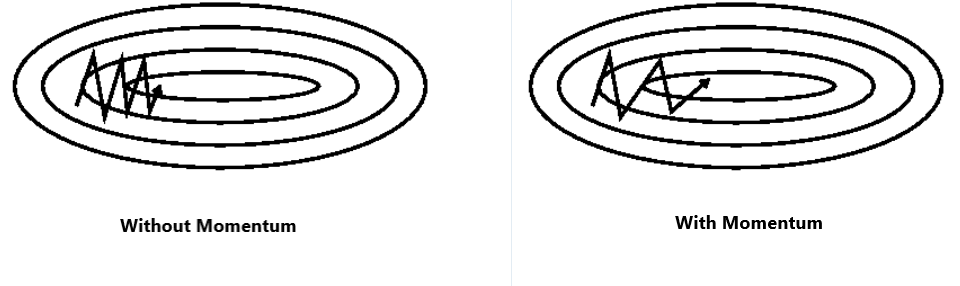
\includegraphics[width=0.80\columnwidth]{Figures/mm.png}
\decoRule
\caption[\textbf{Right:} An optimized gradient descent with momentum. \textbf{Left:} The same gradient descent but without using momentum.]{\textbf{Right:} An optimized gradient descent with momentum. \textbf{Left:} The same gradient descent but without using momentum.}
\label{fig:momentum}
\end{figure}
\begin{equation}\label{eq:eps}
     v=\alpha v-\epsilon \Delta _{\Theta }(\frac{1}{m}\sum _{i}L(f(x^{(i)};\Theta ),y^{(i)}))
\end{equation}

\begin{equation}
    \Theta =\Theta +v
\end{equation}
where $\epsilon$ $\geq$ 0 is the learning rate. Thus step size depends on how large and how aligned the sequence of gradients are.
Equation ~\ref{eq:eps} has two parts. The first term is the gradient that is retained from previous iterations. This retained gradient is multiplied by Coefficient of Momentum $\alpha$ which is the percentage of the gradient retained every iteration.\\

In our experiment, we set the momentum to 0.9 for both of our model. As a result, we gain faster convergence and reduced oscillation.


\section{Summary}
In this chapter, a step by step explanation of our proposed models was given. First, we introduced the popular KTH dataset used for this thesis. Then, we explained our data splits method used to divide the dataset into three main directories. Next, we introduced and explained our first proposed CNN model. In this method, spatial features were extracted where the action of interest is more significant. Then, we introduced and explained our second proposed model CNN-LSTM, which consist of a CNN network combined with a LSTM layer that act as memory layer. At the end, we explained our initialization and optimization method used to make both of these models converge in the global maximum at the end of the training.
%----------------------------------------------------------------------------------------

\chapter{Results and Discussions}

This chapter presents final results of our neural network frameworks. We present graphs, confusion matrices and accuracy \& loss to evaluate our model. We compared the results between these two models. We concluded this chapter with a discussion about the future direction based on the model with highest accuracy and less complexity and computation power.

\section{Results}
In this section we will report the performance of the proposed CNN and CNN-LSTM models on KTH dataset. The performance are compared between both of these models according to their accuracy, loss and confusion matrix.\\

To understand the performance and accuracy of the model, the performance are evaluated using the trained data and perform an evaluation on the test data. Since KTH dataset have similar characteristics, the accuracy would be a suitable metric to evaluate the model. In this case, accuracy is one of our evaluation matrix, it is used to evaluate the performance of the model on the test data, and the confusion matrix is used to compare the model amongst the benchmark model.\\

In practice, accuracy is calculated as the portion of true labeled instances to total number of instances. Both of the models are multi-class classification model. For that reason, the formula for accuracy used is in Equation \ref{accuracymodel}. This equation is well known and it is the standard form of neural network evaluation metrices.

\begin{equation}\label{accuracymodel}
     ACCURACY=\frac{TP+TN}{TP+FP+TN+FN}
\end{equation}
where:\\
\begin{itemize}
    \item \textbf{TP:} True positive
    \item \textbf{TN:} True negative
    \item \textbf{FP:} False positive
    \item \textbf{FN:} False negative
\end{itemize}

Confusion matrix is our second evaluation matrix, it contains information about actual and predicted classifications done by our classification system. Performance of such systems is
commonly evaluated using the data in the matrix. For our experiments a table of confusion, is a table with two rows and two columns that reports the number of FP, FN, TP, and TN, and visualizes the accuracy of each class labels.\\

Loss is our third evaluation matrix. It is a quantitative measure of how much our predictions differ from the actual label. In our experiments, we use the cross entropy loss function. In this case, the formula of cross entropy is presented in Equation \ref{eq:lossfunction}.

\begin{equation}\label{eq:lossfunction}
    H(y,\widehat{y})=\sum _{i}y_{i}log\frac{1}{\widehat{y_{i}}}
\end{equation}
where $\widehat{y_{i}}$ is the ground truth label of the $ith$ training sample, and $y_{i}$ is the prediction result of the classification for the $ith$ training instance. During training, the cross entropy $\sum _{i}y_{i}$ is minimised.\\

The evaluation results are provided in the Table \ref{table:finalresults}.
\begin{figure}[ht]
\centering
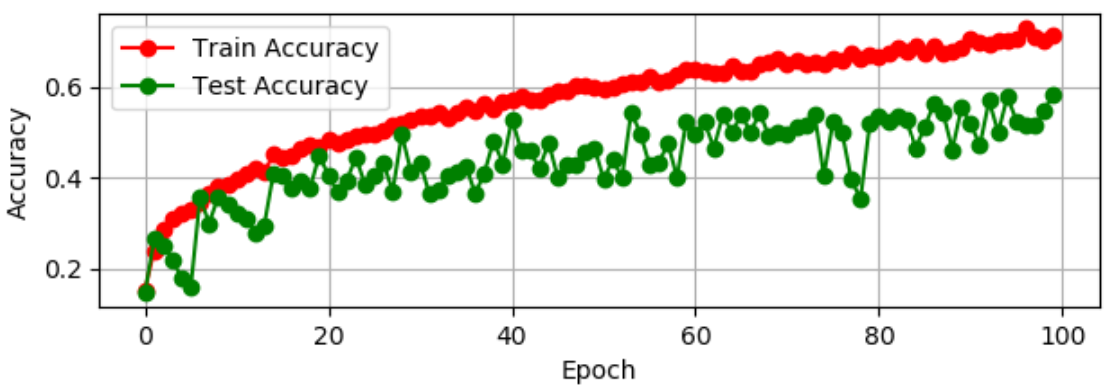
\includegraphics[width=1.0\columnwidth]{Figures/accuracycnnmodel}
\decoRule
\caption[The accuracy of the first convolutional neural network model.]{The accuracy of the first convolutional neural network model.}
\label{fig:cnnaccuracy12}
\end{figure}

Figure \ref{fig:cnnaccuracy12} shows the accuracy of the CNN model across the training and test set. The model was trained on the training data for 100 epochs. The weights of the model which gave the test performance on the validation data were loaded. The model was then tested on the test data. After training the model gave an accuracy of approximately 64.76\% on the training set, while it achieved an accuracy of 60\% on the validation set.


\begin{figure}[ht]
\centering
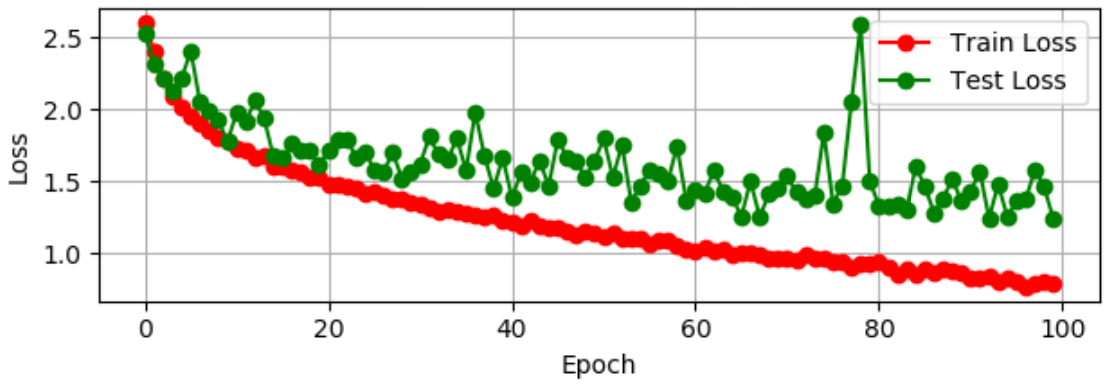
\includegraphics[width=1.0\columnwidth]{Figures/losscnnmodel}
\decoRule
\caption[A visualization of the Loss of the first convolutional neural network model.]{A visualization of the Loss of the first convolutional neural network model.}
\label{fig:cnnaccuracy13}
\end{figure}

Figure \ref{fig:cnnaccuracy13} represents the model loss across the training and test set. These values were calculated according to Equation \ref{eq:lossfunction} above. The results shows that the model achieved a loss of 0.823 on the training set and approximately 1.032 on the validation set.\\

As we can observe from the learning curve from Figure \ref{fig:cnnaccuracy12} and Figure \ref{fig:cnnaccuracy13}, the difference in results between train and test set are not significant, although training set performs slightly better. The training accuracy across the test set were not stable specially at the beginning of the training from 0 to the $18^{th}$ epochs and between the $75^{th}$ and $80^{th}$ epochs. Here, it means that although the model performed better on the training data, but its performance on the validation data get degraded. This is because the model is too complex for the data and it starts to memorize the training data. The same pattern appear on the model loss. Both of the training and test set were having nearly same loss, the training set continue decrease steeply. After that, the model shows over-fitting on the validation set between the $75^{th}$ and $80^{th}$, here the loss dramatically increases. At the end of the training  and after the $80^{th}$ epoch, the model shows good loss results.


\begin{figure}[ht]
\centering
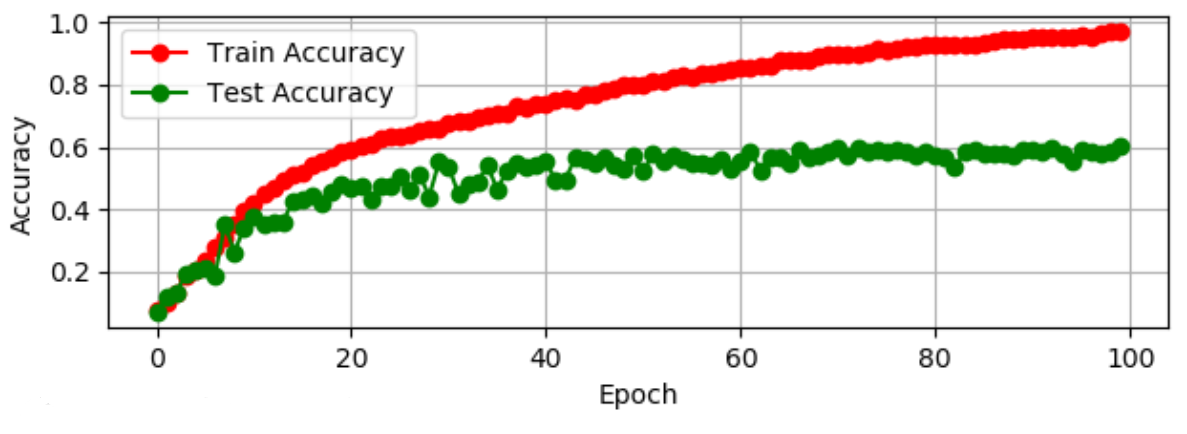
\includegraphics[width=1.0\columnwidth]{Figures/accuracycnnlstmmodel}
\decoRule
\caption[The accuracy of the second convolutional long short term memory neural network model.]{The accuracy of the second convolutional long short term memory neural network model.}
\label{fig:accuracycnnlstmmodel} 
\end{figure}

Figure \ref{fig:accuracycnnlstmmodel} represents the accuracy of the second CNN-LSTM model, which is trained over 100 epochs. In this model the weights that gives the best performance on the validation data were loaded. After that, the model is tested on the test set. At the end of the training, the model gave an accuracy of 92.23\% on the training set and 61.2\% of the test set. The current results are an improvement of 27.47\% from the previous architecture.

\begin{figure}[ht]
\centering
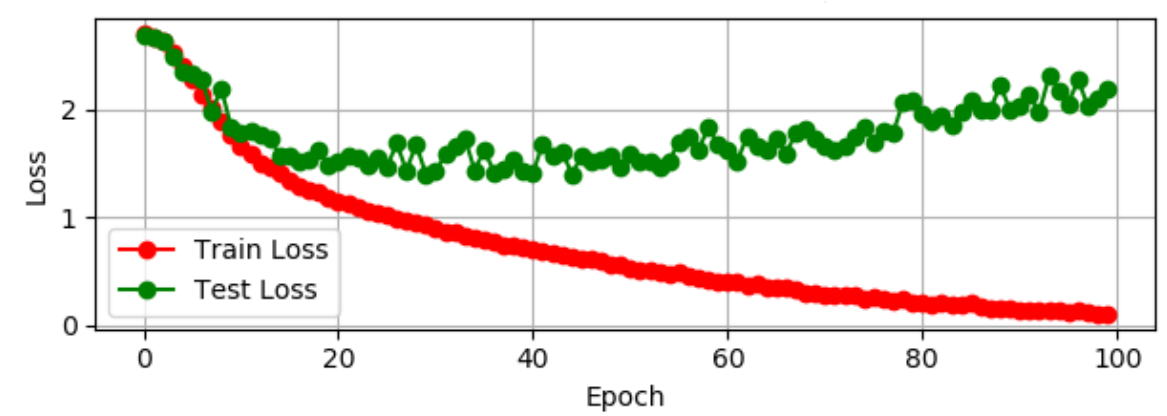
\includegraphics[width=1.0\columnwidth]{Figures/losscnnlstmmodel}
\decoRule
\caption[A visualization of the Loss of the second convolutional long short term memory neural network model.]{A visualization of the Loss of the second convolutional long short term memory neural network model.}
\label{fig:losscnnlstmmodel}
\end{figure}

Figure \ref{fig:losscnnlstmmodel} shows the model loss on the training and test set. This architecture successfully scored a loss of 0.087 on the training set and nearly 2.1 on the test set. This is because the model performed better on the training data, but failed to perform good on the test set, due to the data complexity and variation in the pattern in each frame.\\

As we can observe from the learning curve from figure \ref{fig:accuracycnnlstmmodel} and figure \ref{fig:losscnnlstmmodel}, that the training is more stable than the previous CNN model. However, the model loss did not perform well on the test set, as it shows large differences between the training and test. Overall, final results show that with much deeper model and less parameters, the model is morel likely to perform better and generate more accurate prediction, than a model with less network and more parameters, as it is shown in table \ref{table:finalresults}.
\begin{table}[ht]
\caption{Final results for the CNN and CNN-LSTM model.}
\centering
\begin{tabular}{|c|c|c|c|c|}
\hline
\textbf{Model name} & \textbf{Accuracy} & \textbf{Loss} & \textbf{Layers} & \textbf{Parameters} \\ \hline
\textbf{CNN} & 64.76\% & 0.823 & 13 & 8,543,110 \\ \hline
\textbf{CNN-LSTM} & 92.23\% & 0.087 & 18 & 1,657,792 \\ \hline
\end{tabular}

\label{table:finalresults}
\end{table}\\

%-Confusion matrix----------------------------------------------------------------------------------

Figure \ref{fig:cmsnnlstm}, Figure \ref{fig:cmcnn} and Figure \ref{fig:cmbm} show the confusion matrix of the proposed CNN-LSTM model, the proposed CNN model and the benchmark results released by KTH authors. Technically, the confusion matrix was implemented by randomly selecting 9 different videos from the dataset, then processed these video than consist of different action labels. In this process, all confusion matrix have been converted in the same format, and they have been normalized. We look at the diagonal line in the diagram which shows the accuracy of each particular action labels. In case of Walking, when the actual label was "walking", the benchmark predicted the label 74\% of the time, whereas the proposed models predicted 84\% and 94\% for the CNN and CNN-LSTM respectively. A higher value was scored by the CNN model. In case of Handwaving, when the actual label was "Handwaving", the benchmark predicted the label 55\% of the time, whereas the proposed models predicted 72\% and 74\% for the CNN and CNN-LSTM respectively. A higher value was scored by the CNN-LSTM model. In case of Jogging, when the actual label was "Jogging", the benchmark predicted the label 98\% of the time, whereas the proposed models predicted 69\% and 60\% for the CNN and CNN-LSTM respectively. A higher value was scored by the benchmark model. This suggest that the proposed model was better at predicting jogging action better than the our proposed model. Another interesting pattern appeared in handclapping action, where the proposed CNN model predict this action 100\% all the time, whereas the 60\% of the time for the CNN-LSTM and the benchmark results. That's mean that the model successfully distinguished handclapping from all other activities and had 'no confusion' when giving a prediction about this action. However, for the remaining action like boxing, the CNN model predicted it 14\% and 98\% of the time for the CNN-LSTM model, in this case there are a huge gap between the two models. This means that videos in which action being performed was boxing were predicted by our proposed model with a better recognition rate than that of the benchmark model.\\

Overall, the CNN model scored a high recognition value for "Walking", "Handclapping" and "Running", whereas the CNN-LSTM achieved a high recognition rate for "Handwaving" and "boxing". Both of the model surpassed the benchmark results. In Figure \ref{fig:classified1} and Figure \ref{fig:missclassified1} we present our final prediction on some random frames, we showed the well classified and the miss-classified results. 
\begin{figure}[ht]
\centering
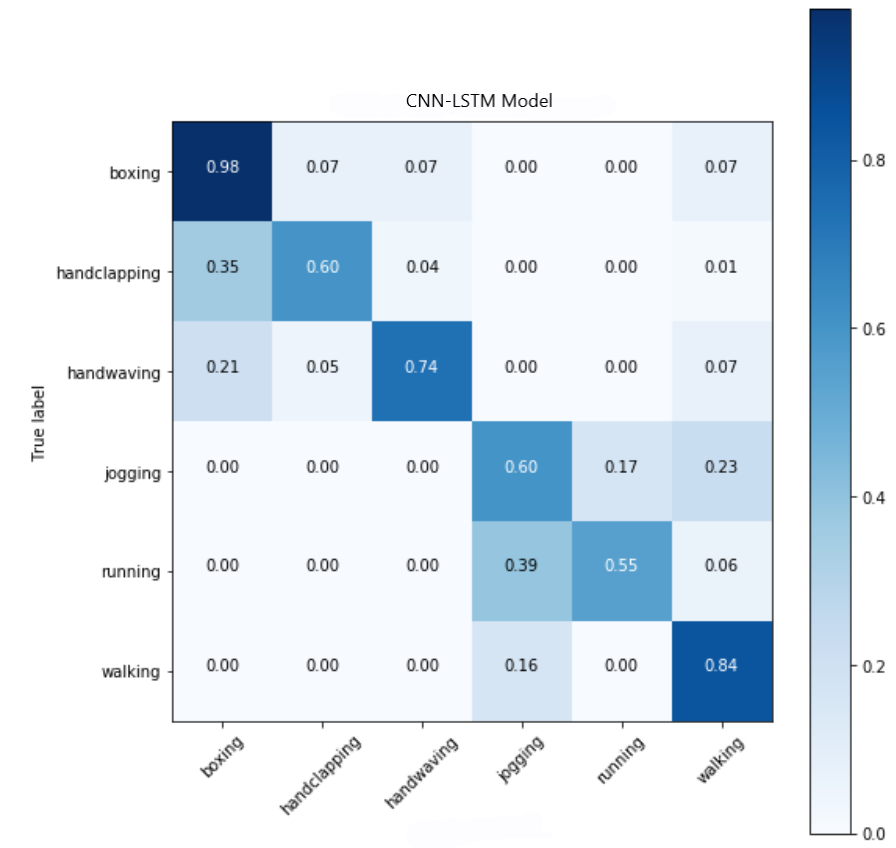
\includegraphics[width=1.0\columnwidth]{Figures/cnnlstmodel.png}
\decoRule
\caption[A visualization of the confusion matrix results for the proposed CNN-LSTM model.]{A visualization of the confusion matrix results for the proposed CNN-LSTM model.}
\label{fig:cmsnnlstm}
\end{figure}


\begin{figure}[ht]
\centering
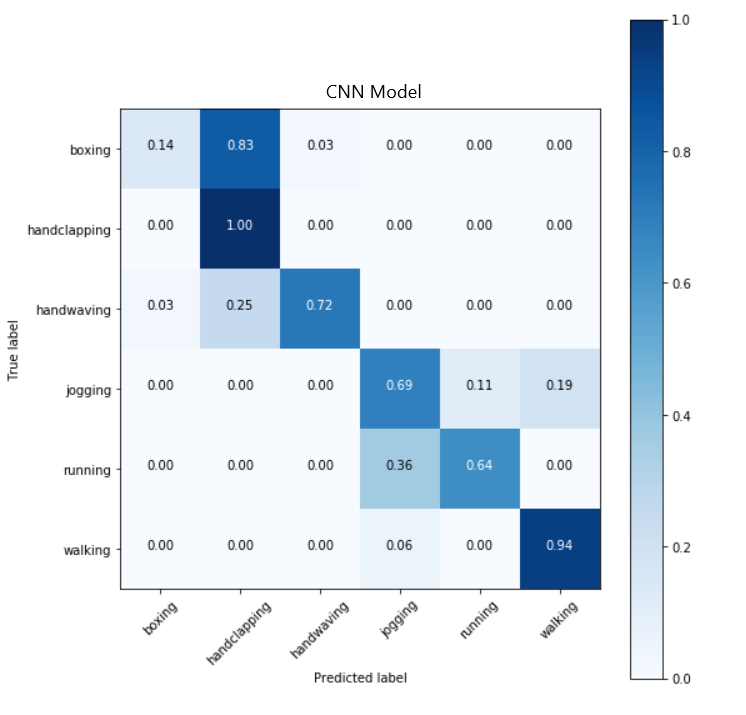
\includegraphics[width=1.0\columnwidth]{Figures/benchmarkresult.png}
\decoRule
\caption[A visualization of the confusion matrix results for the proposed CNN model.]{A visualization of the confusion matrix results for the proposed CNN model.}
\label{fig:cmcnn}
\end{figure}


\begin{figure}[ht]
\centering
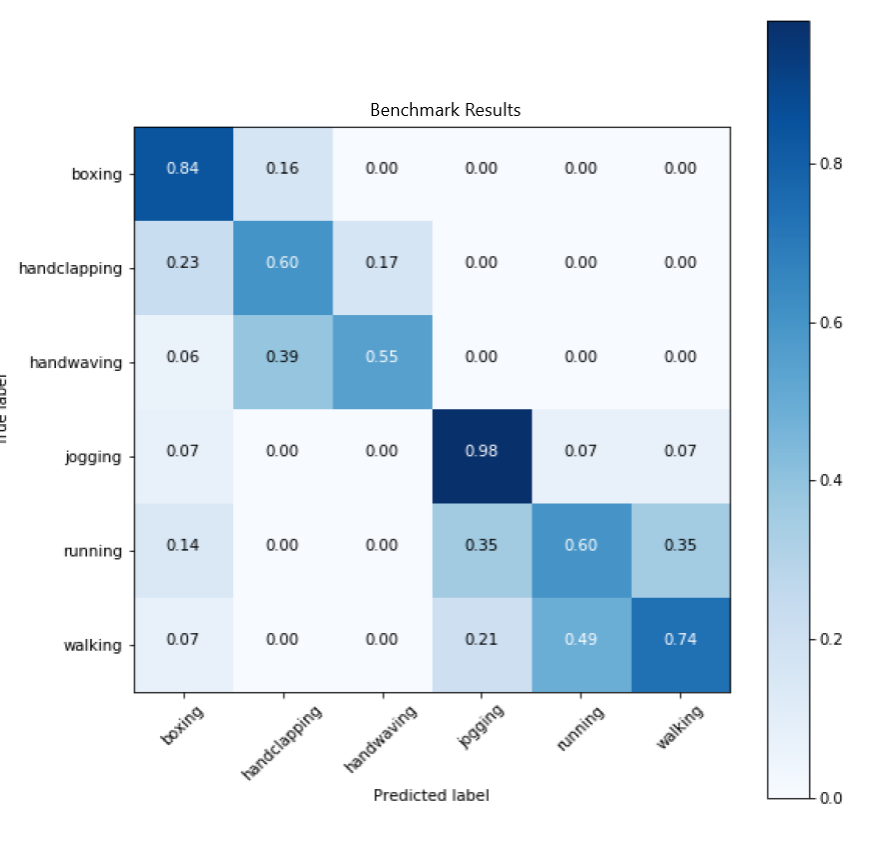
\includegraphics[width=1.0\columnwidth]{Figures/bm.png}
\decoRule
\caption[A visualization of the confusion matrix for benchmark results, released by KTH dataset authors.]{A visualization of the confusion matrix for benchmark results, released by KTH dataset authors.}
\label{fig:cmbm}
\end{figure}

\begin{table}[ht]
\caption{A table represents a summary of the results taken from the confusion matrix.}

\centering
\begin{tabular}{|c|c|c|c|}
\hline
\textbf{Action} & \textbf{CNN model} & \textbf{CNN-LSTM} & \textbf{Benchmark} \\ \hline
\textbf{Walking} & 94\% & 84\% & 74\% \\ \hline
\textbf{Jogging} & 69\% & 60\% & 98\% \\ \hline
\textbf{Handclapping} & 100\% & 60\% & 60\% \\ \hline
\textbf{Handwaving} & 72\% & 74\% & 55\% \\ \hline
\textbf{Running} & 64\% & 55\% & 60\% \\ \hline
\textbf{Boxing} & 14\% & 98\% & 84\% \\ \hline
\end{tabular}
\label{my-label}
\end{table}\\

\begin{table}[]
\caption{We represent the summary of the confusion matrix results.}
\centering
\begin{tabular}{|c|c|c|c|}
\hline
\textbf{Action} & \textbf{CNN model} & \textbf{CNN-LSTM} & \textbf{Benchmark} \\ \hline
\textbf{Walking} & Better & - & - \\ \hline
\textbf{Jogging} & - & - & Better \\ \hline
\textbf{Handclapping} & Better & - & - \\ \hline
\textbf{Handwaving} & - & Better & - \\ \hline
\textbf{Running} & Better & - & - \\ \hline
\textbf{Boxing} & - & Better & - \\ \hline
\end{tabular}

\label{my-label}
\end{table}

\begin{figure}[ht] 
\centering
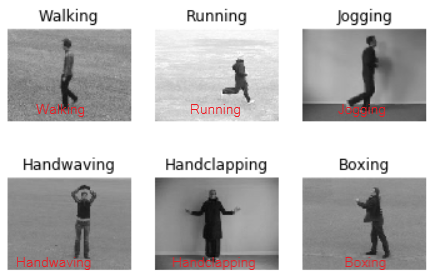
\includegraphics[width=1.0\columnwidth]{Figures/classified.png}
\decoRule
\caption[Visualization of the correctly classified action samples.]{Visualization of the correctly classified action samples.}
\label{fig:classified1}
\end{figure}


\begin{figure}[ht]
\centering
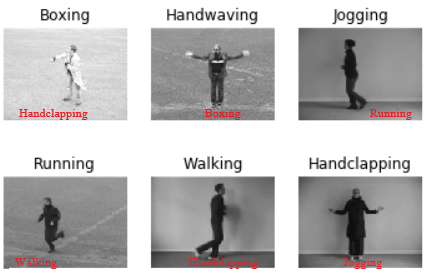
\includegraphics[width=1.0\columnwidth]{Figures/missclassified.png}
\decoRule
\caption[Visualization of the miss classified action samples.]{Visualization of the miss classified action samples.}
\label{fig:missclassified1}
\end{figure}
%----------------------------------------------------------------------------------------
After evaluating our model against the benchmark results, we wanted to know where we stand against other implementations and methods. Therefore, we have conducted an in-depth analysis and collected 29 papers that used the same KTH dataset type and we classified them in term of accuracy and year published and at the end we made a comparison for the same paper that used the same method as us. In Table ~\ref{table:finalresults} we have showed 29 papers; we have showed the authors name, year, method used and the accuracy achieved. Refer to Figure ~\ref{fig:accuracycomparison}, Figure ~\ref{fig:accuracycomparison1} and Figure ~\ref{fig:accuracycomparison2} for visualization. We have highighted our method with red to provide more insight.
%Possible future research directions that could be pursued as a natural extensions of this work are also pointed out.

% Please add the following required packages to your document preamble:
% \usepackage[table,xcdraw]{xcolor}
% If you use beamer only pass "xcolor=table" option, i.e. \documentclass[xcolor=table]{beamer}
% \usepackage{longtable}
% Note: It may be necessary to compile the document several times to get a multi-page table to line up properly
\begin{longtable}[c]{|c|c|c|c|}
\caption{An overview of previous papers and work in the HAR field.}
\label{PreviousResults}\\
\hline
\textbf{Author}                                                  & \textbf{Year}               & \textbf{Method}                                                                                 & \textbf{Accuracy}             \\ \hline
\endhead
%
\textbf{Our Method}                                              & {\color[HTML]{000000} 2019} & {\color[HTML]{000000} \begin{tabular}[c]{@{}c@{}}CNN -\\   RNN network\end{tabular}}            & {\color[HTML]{000000} 92.23\%} \\ \hline
\begin{tabular}[c]{@{}c@{}}\cite{laptev2004recognizing}\end{tabular}      & {\color[HTML]{000000} 2004} & {\color[HTML]{000000} \begin{tabular}[c]{@{}c@{}}Local\\   Feature, SVM\end{tabular}}           & {\color[HTML]{000000} 78\%}    \\ \hline
\begin{tabular}[c]{@{}c@{}}\cite{laptev2004recognizing}\end{tabular}      & 2004                        & Histogram Local Feature                                                                         & 75\%                           \\ \hline
\begin{tabular}[c]{@{}c@{}}\cite{laptev2004recognizing}\end{tabular}      & 2004                        & Histogram STG                                                                                   & 75.50\%                        \\ \hline
\begin{tabular}[c]{@{}c@{}}\cite{laptev2004recognizing}\end{tabular}      & 2004                        & \begin{tabular}[c]{@{}c@{}}Histogram\\   LF\end{tabular}                                        & 70\%                           \\ \hline
\begin{tabular}[c]{@{}c@{}}\cite{laptev2004recognizing}\end{tabular}      & 2004                        & \begin{tabular}[c]{@{}c@{}}Histogram\\   STG\end{tabular}                                       & 67\%                           \\ \hline
\cite{moussa2015enhanced}                                                  & 2015                        & \begin{tabular}[c]{@{}c@{}}SIFT\\   \end{tabular}            & 97.89\%                        \\ \hline
\begin{tabular}[c]{@{}c@{}}\cite{bregonzio2012fusing}\end{tabular}     & 2012                        & \begin{tabular}[c]{@{}c@{}}Feature\\   Fusion\end{tabular}                                      & 94.33\%                        \\ \hline
\begin{tabular}[c]{@{}c@{}}\cite{liu2008learning}\end{tabular}         & 2008                        & \begin{tabular}[c]{@{}c@{}}Bag of\\   video-words\end{tabular}                                  & 94.20\%                        \\ \hline
\begin{tabular}[c]{@{}c@{}}\cite{lin2009recognizing}\end{tabular}           & 2009                        & \begin{tabular}[c]{@{}c@{}}Prototype-based\\   approach\end{tabular}                            & 93.43\%                        \\ \hline
\begin{tabular}[c]{@{}c@{}}\cite{chen2009mosift}\end{tabular}    & 2009                        & MoSIFT                                                                                          & 95.83\%                        \\ \hline
\begin{tabular}[c]{@{}c@{}}\cite{niebles2008unsupervised}\end{tabular}       & 2008                        & \begin{tabular}[c]{@{}c@{}}Spatial-Temporal\\   Words\end{tabular}                              & 95.83\%                        \\ \hline
\begin{tabular}[c]{@{}c@{}}\cite{tran2011modeling}\end{tabular}          & 2011                        & \begin{tabular}[c]{@{}c@{}}Pictorial\\   structures model\end{tabular}                          & 95.67\%                        \\ \hline
\begin{tabular}[c]{@{}c@{}}\cite{fathi2008action}\end{tabular}       & 2008                        & \begin{tabular}[c]{@{}c@{}}Low-level\\   optical flow\end{tabular}                              & 90.50\%                        \\ \hline
\begin{tabular}[c]{@{}c@{}}\cite{kovashka2010learning}\end{tabular} & 2010                        & \begin{tabular}[c]{@{}c@{}}Space-time\\   feature\\ neighborhoods\end{tabular}                    & 94.53\%                        \\ \hline
\begin{tabular}[c]{@{}c@{}}\cite{cao2010cross}\end{tabular}           & 2010                        & \begin{tabular}[c]{@{}c@{}}Maximum\\   a Posterior (MAP)\\  estimation\end{tabular}                & 95.02\%                        \\ \hline
\begin{tabular}[c]{@{}c@{}}\cite{kaaniche2010gesture}\end{tabular} & 2010                        & \begin{tabular}[c]{@{}c@{}}Local\\   motion signatures (LMSs)\end{tabular}                      & 94.67\%                        \\ \hline
\begin{tabular}[c]{@{}c@{}}\cite{dollar2005behavior}\end{tabular}        & 2005                        & \begin{tabular}[c]{@{}c@{}}Spatial\\   and temporall features\end{tabular}                      & 81.17\%                        \\ \hline
\begin{tabular}[c]{@{}c@{}}\cite{klaser2008spatio}\end{tabular}        & 2010                        & \begin{tabular}[c]{@{}c@{}}Histograms\\   of oriented 3D \\ spatio-temporal gradients\end{tabular} & 91.40\%                        \\ \hline
\begin{tabular}[c]{@{}c@{}}\cite{klaser2008spatio}\end{tabular}         & 2008                        & \begin{tabular}[c]{@{}c@{}}Motion\\   Context (MC)\end{tabular}                                 & 91.33\%                        \\ \hline
\begin{tabular}[c]{@{}c@{}}\cite{rodriguez2010spatio}\end{tabular}     & 2010                        & \begin{tabular}[c]{@{}c@{}}Maximum\\   average\\     correlation height\\  filter\end{tabular}     & 80.90\%                        \\ \hline
\begin{tabular}[c]{@{}c@{}}\cite{ke2005efficient}\end{tabular}            & 2005                        & Adaboost                                                                                        & 62.97\%                        \\ \hline
\begin{tabular}[c]{@{}c@{}}\cite{laptev2008learning}\end{tabular}        & 2008                        & Support Vector Machine - SVM                                                                    & 91.80\%                        \\ \hline
\begin{tabular}[c]{@{}c@{}}\cite{wang2011action}\end{tabular}          & 2011                        & \begin{tabular}[c]{@{}c@{}}Dense\\   trajectory\\  with HOG, HOF, MBH\end{tabular}                 & 94.20\%                        \\ \hline
\begin{tabular}[c]{@{}c@{}}\cite{wang2011action}\end{tabular}          & 2012                        & \begin{tabular}[c]{@{}c@{}}STIP\\   with HOG, HOF\end{tabular}                                  & 92.13\%                        \\ \hline
\begin{tabular}[c]{@{}c@{}}\cite{grushin2013robust}\end{tabular}       & 2013                        & RNN with  LSTM                                                                                  & 90.70\% \\ \hline
\begin{tabular}[c]{@{}c@{}}\cite{wang2011action}\end{tabular}          & 2015                        & \begin{tabular}[c]{@{}c@{}}Differential\\   Recurrent Neural\\  Network (dRNN)\end{tabular}        & 93.96\% \\ \hline
\begin{tabular}[c]{@{}c@{}}\cite{zhen2016action}\end{tabular}          & 2016                        & \begin{tabular}[c]{@{}c@{}}STIP\\   with HOG3D\end{tabular}                                     & 94.10\%                        \\ \hline
\begin{tabular}[c]{@{}c@{}}\cite{shi2017sequential}\end{tabular}           & 2016                        & RNN and Deep ConvNets                                                                           & 96.80\%                        \\ \hline
\end{longtable}



\begin{figure}[ht]
\centering

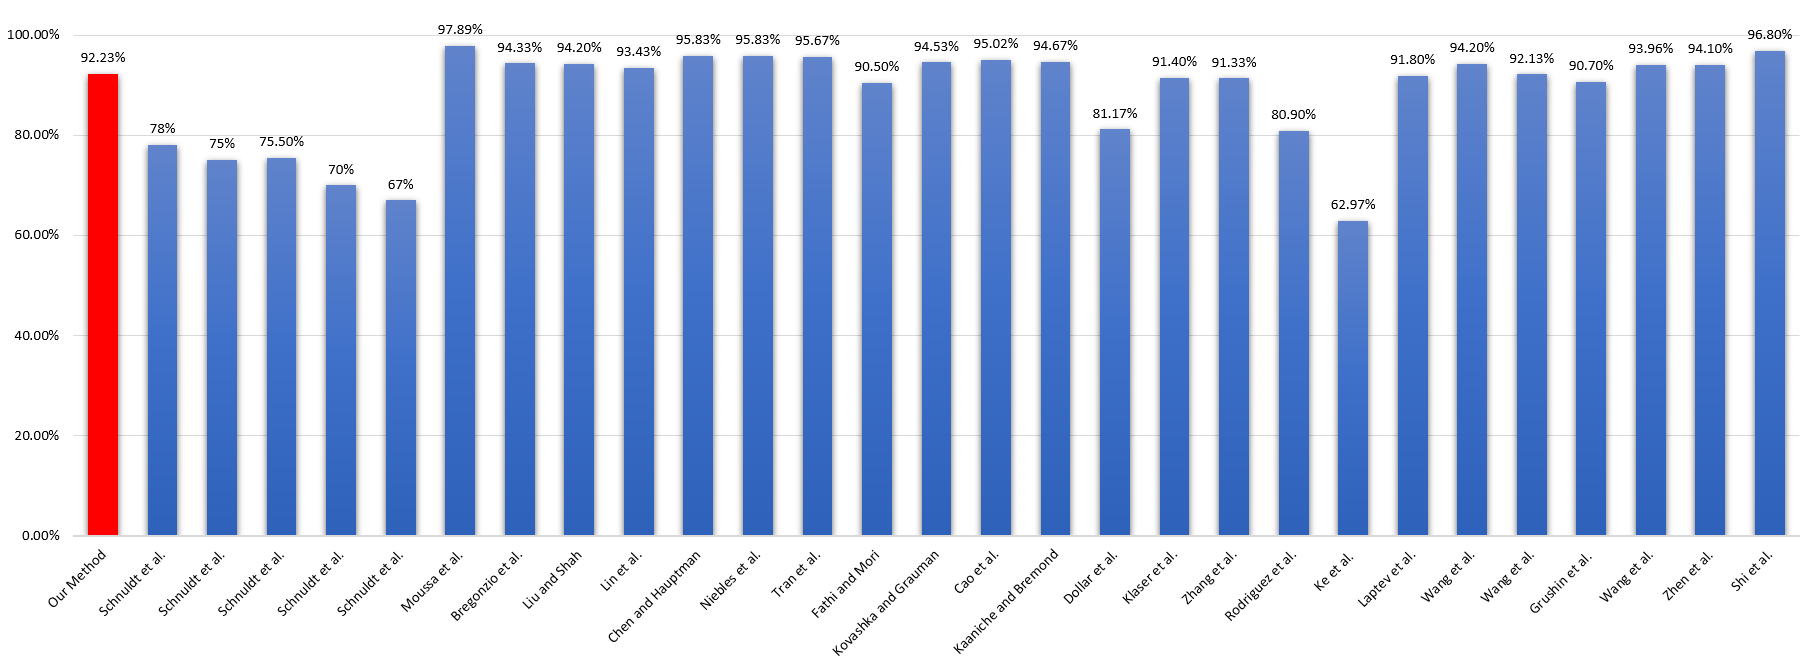
\includegraphics[angle=90,origin=c,width=0.6\columnwidth]{Chapters/photos/comparisonintermofaccuracy.PNG}

\decoRule
\caption[A comparison of our method against other papers in term of accuracy.]{A comparison of our method against other papers in term of accuracy.}
\label{fig:accuracycomparison}
\end{figure}



\begin{figure}[ht]
\centering
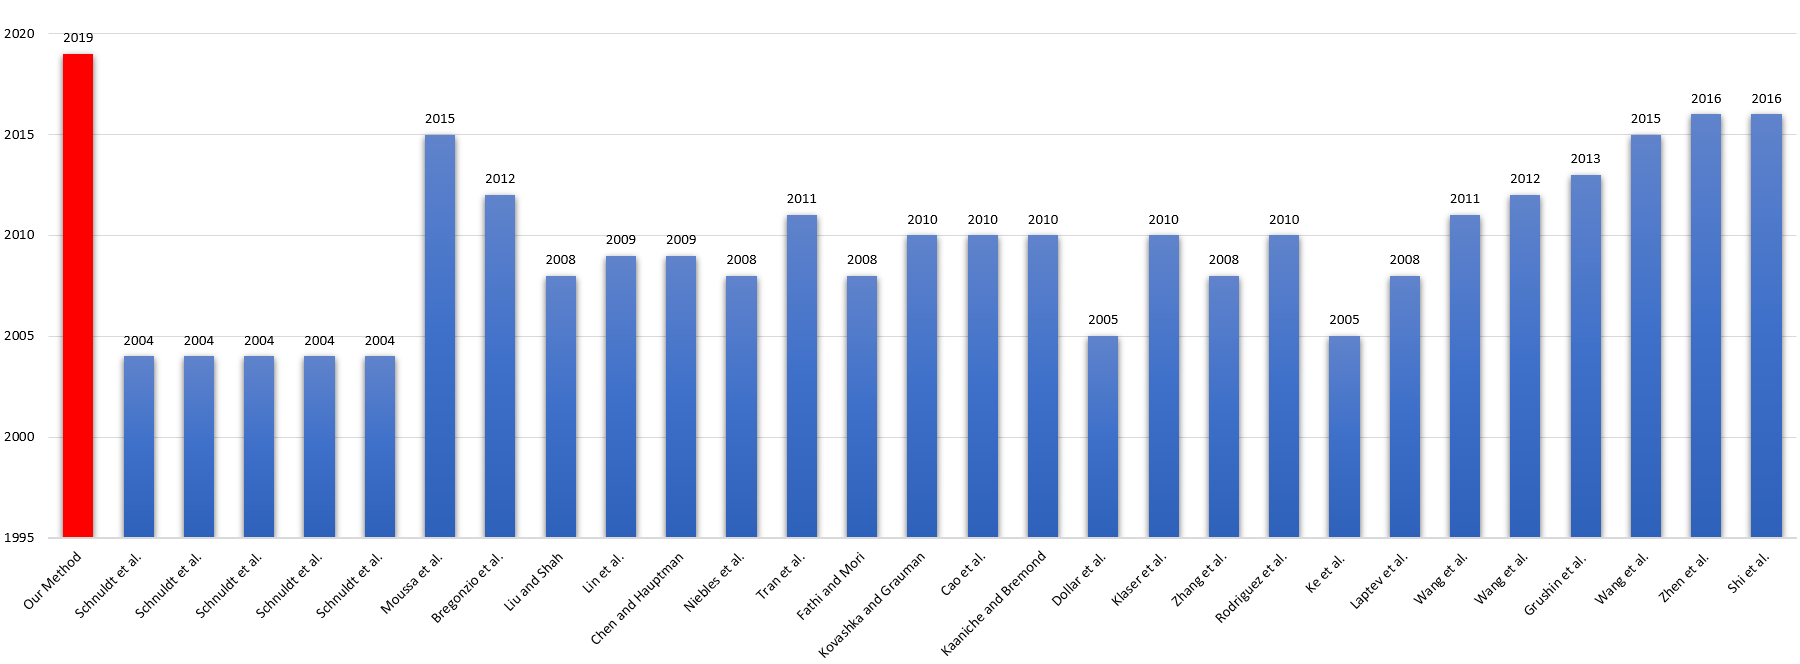
\includegraphics[angle=90,origin=c,width=0.6\columnwidth]{Chapters/photos/comparisonintermofyear.PNG}
\decoRule
\caption[A comparison of our method against other papers in term of year published.]{ comparison of our method against other papers in term of year published.}
\label{fig:accuracycomparison1}
\end{figure}

\begin{figure}[ht]
\centering
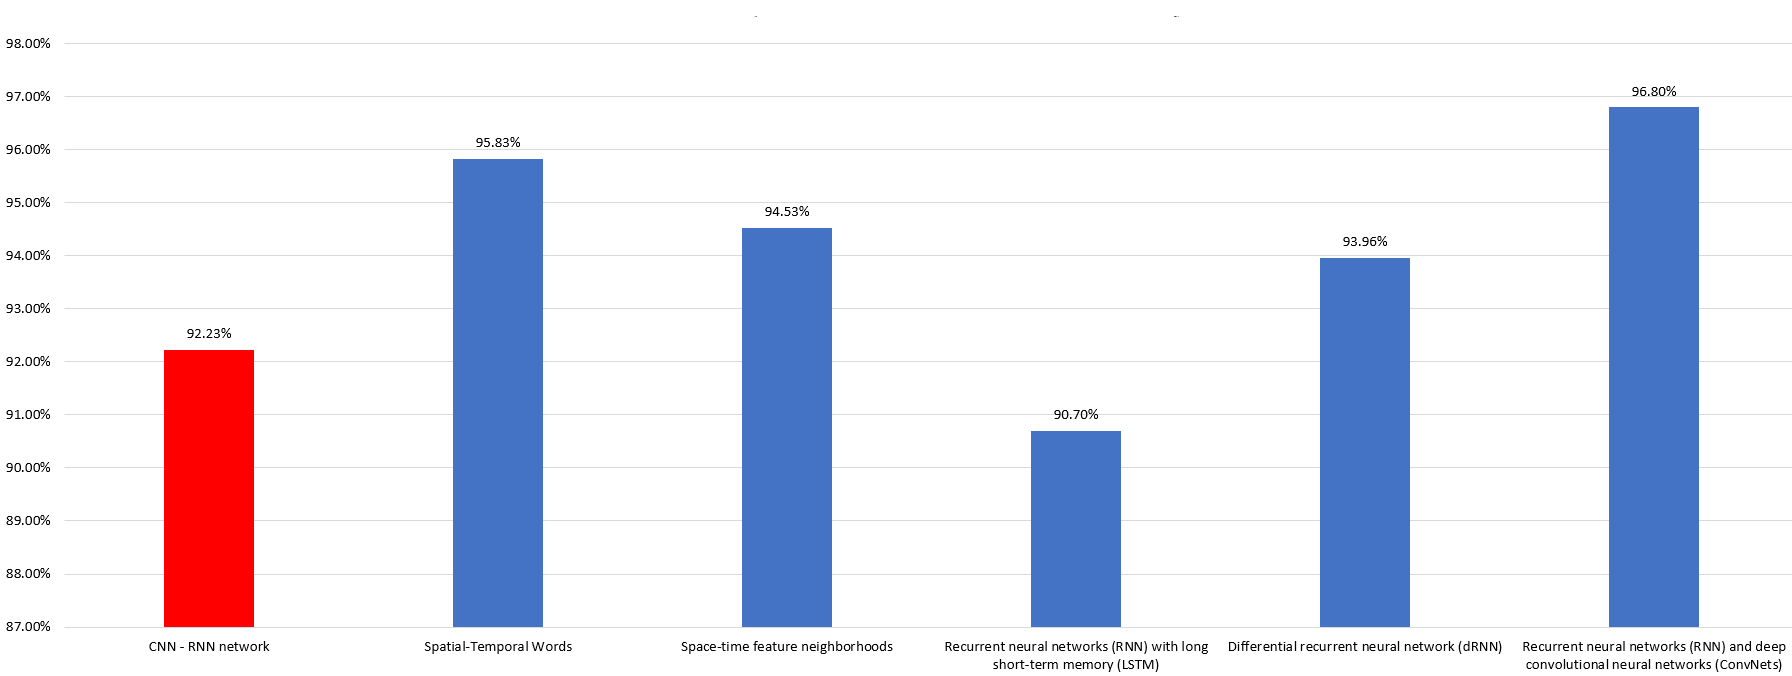
\includegraphics[angle=90,origin=c,width=0.6\columnwidth]{Chapters/photos/comparisonintermofCNNRNN.PNG}
\decoRule
\caption[A comparison of our method against other papers in term of method.]{ comparison of our method against other papers in term of method.}
\label{fig:accuracycomparison2}
\end{figure}
\section{Summary}
In this chapter we represent our network performance. We proposed 2 methods: a method that encodes spatial information using CNN layers and regularization and a method that encode the same information with an additional memory architecture added to the model, where spatial and temporal features are concatenated and trained to predict the label of a particular sequence.
The CNN takes advantage of implicit posture information and it is able to efficiently encode spatial information. While the other model predict the action based on a sequence of frame using recurrent gates.
Final experimental results shows that the proposed models surpassed benchmark results significantly. The CNN model was able to recognize three action higher than any other model, while the CNN-LSTM was able to score a high value for two actions.

Finally we would like to highlight that propose spatial layout encoding methods improve both hand-crafted and CNN based representation and lead to significant improvements in recognition accuracy.
%----------------------------------------------------------------------------------------

\chapter{Conclusion and Recommendations}

This chapter presents a summary of the work presented in this thesis and the conclusions drawn from it, and a brief conclusion of research gaps, research objectives, the methods used and their obtained results. Even though several activity recognition frameworks exist in the previous literature, memory-based systems are very popular due to their simplicity and their superior performance. In this thesis, feature-based and memory-based action recognition has been extensively studied and several advances have been proposed. The summary follows the three main research themes and areas of contribution in providing a comprehensive evaluation of the feature-based action recognition system, improving the system performance by developing new, efficient spatio-temporal features and developing new feature representation and classification architecture to improve the overall recognition performance amongst benchmarks. Possible future research directions that could be pursued as a natural extensions of this work are also pointed out. 

\section{Limitations and Research gaps}
The methods proposed in this thesis have still some limitations. Some of them can be seen
as extensions and can be solved in near future. While others are still open questions. In this section we present the limitations and research gaps.\\

The method proposed and the data used in this thesis assumes that there is only one person in the scene. In real-world scenarios, more people might be present on the scene. In particular some action involves more than one person,  this case is not covered by the proposed method. Modeling spatial layout that only rely on people appearance may not work when actions are done by multiple humans, where multiple actions are performed by many people that looks the same. In addition our Mixture of CNN and RNN concentrates too much on areas with high action of interest, which limits it’s performance in real world scenario.\\

Unconstrained action recognition from “real-world” videos,
however, remains a challenging problem. State-of-the-art
methods are currently very far from the perfect scores obtained by systems developed for image classification due to activity complexity, insufficient training set and personal biometric signature. This fact is underscored by the properties of the benchmarks
used to develop, train, and test systems for action recognition in videos, compared to systems for image classification, where the latter include hundreds of action categories and labels,
peaking at thousands of video samples, the former provide
thousands of categories and millions of photo samples. This
is particularly troubling when considering that actions can
vary greatly in how they appear in videos, and that most of the people appear to perform action that is even confusing to be recognized by human, possibly far more
than static items vary in appearance in photos, implying that
data sets for action recognition must be designed to offer
more examples and cover many scenarios with less computation power.

\section{Future Work}
This thesis contribute to the field of human action recognition. Given these contribution, it is important that the works continues to improve and develop to provide further applications in human activity recognition and advance the field of computer vision further.\\

It is suggested that the feature-based CNN methodology introduced in Chapter 2, could be improved by removing the limitation of number of frames selected per activity. This would allow activities that have more motion present to have more features while activities with fewer movements can be represented by fewer features. A second suggestion could be to adopt a bounding box based approach by modelling the features
inside a particular box for each region in the frame. This could prove useful to provide a better model of more localised activities.\\

The second activity recognition approach introduced in the same Chapter could be improved by adding the tracking approach. The action can be then detected more robustly and the long term changes in motion and location would also be modelled. A further suggestion is to modify the proposed concatenation methodology either by using a depth estimation to determine the approximate distance of the pedestrians from the camera, or by fusing the CNN model and LSTM with Generative adversarial network (GAN) that generator predict action labels and the discriminator distinguish between the real prediction and the fake one. The performance can also be improved by introducing attentions mechanism to the network, we believe that long, complex action recognition or action detection can be improved with attention mechanism. Such mechanism lets the algorithm focus on important subsequences of action.\\

Finally, I suggested to adopt the bounding box approach for both of the methods introduced in Chapter 2. This method is intended to focus on the human as object of interest and the proposed model is applied to down sample the video before being fed to the neural network then automatically predict its associated labels. I also plan to use Depth sensor to introduce the depth as a new set of information; this information will allow the system to learn more about the video, and therefore, produce more accurate results. 

\section{Conclusion}
This thesis proposed and examined two deep neural network architectures and proved that they can be used for human action recognition in video sequences. The widely know AlexNet CNN architecture was intensified with different regularization layers to improve action predictions that make use of several frames of video for their recognition. The motivation is that when a single-frame feedforward neural network is used to distinguish actions in videos the resulting actions trajectory is noisy and requires postprocessing. A recurrent neural network can learn to track activity across multiple frames as a result of the learning and produce smoother detections. A convolutional multiple-frame action detector neural network acted as a baseline model for all comparisons.\\

The experiments measured the models’ performance under varying levels of scenarios applied to the videos dataset such as zooming, light effect, outdoor and indoor etc. The results showed that the recurrent architectures outperform the CNN action detector model and are more robust to variation and noise. The models are also more confident in their predictions. The recurrent architectures also defeat and outperform the benchmark model in action detection tasks as they form a temporal context across several frames of video.\\

A set of recurrent models was examined and it is likely that the choices of learning rate, activation functions, kernel sizes, layer count, etc. were not optimal for this problem. The interactions between hyper-parameters can be difficult to predict and the difficulty increases with every distinct hyper-parameter. Finding the optimal architecture and parametrization for this problem was left for future research. Neural networks are complex nonlinear models and creating them requires an instinctive high-level understanding of the learning dynamics. This thesis gave some practical insights into choosing the network structure, learning rate and other hyper-parameters. However, the field of deep learning is developing rapidly and more concrete guidelines for neural network design are apparent to arrive in the future. In the end, it is noteworthy that the experimenter evaluates many models suitable for their particular problem.\\




\chapter{Project Timeline}

\begin{figure}[ht]
\centering

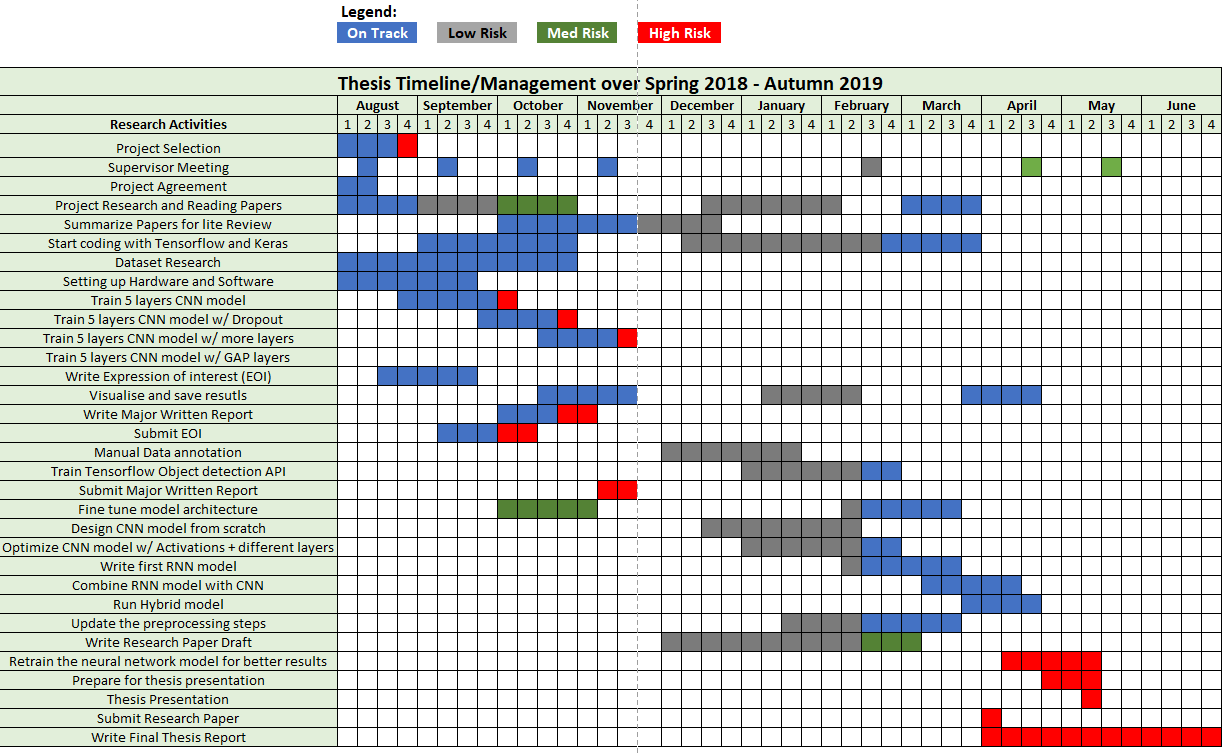
\includegraphics[angle=90,origin=c,width=0.7\columnwidth]{Figures/Project_Timeline.PNG}
\decoRule
\caption[Engineering Thesis 1 \& 2 Gantt Chart: Illustrate the tasks performed between Spring 2018 - Autumn 2019.]{Engineering Thesis 1 \& 2 Gantt Chart: Illustrate the tasks performed between Spring 2018 - Autumn 2019.}
\label{fig:missclassified1}
\end{figure}

\section{Appendices}

\lstinputlisting[
	caption= Python implementation of our second proposed neural network model CNN-LSTM, % Caption above the listing
	label=lst:luftballons, % Label for referencing this listing
	language=Python, % Use Perl functions/syntax highlighting
	frame=single, % Frame around the code listing
	showstringspaces=false, % Don't put marks in string spaces
	numbers=left, % Line numbers on left
	numberstyle=\tiny, % Line numbers styling
	]{Chapters/code/appendices1.py}
	
\lstinputlisting[
	caption= Script to visualize all the feature map in the convolutional and maxpoolingl layers, % Caption above the listing
	label=lst:luftballons, % Label for referencing this listing
	language=Python, % Use Perl functions/syntax highlighting
	frame=single, % Frame around the code listing
	showstringspaces=false, % Don't put marks in string spaces
	numbers=left, % Line numbers on left
	numberstyle=\tiny, % Line numbers styling
	]{Chapters/code/appendices2.py}
	
	
\begin{figure}[ht]
\centering
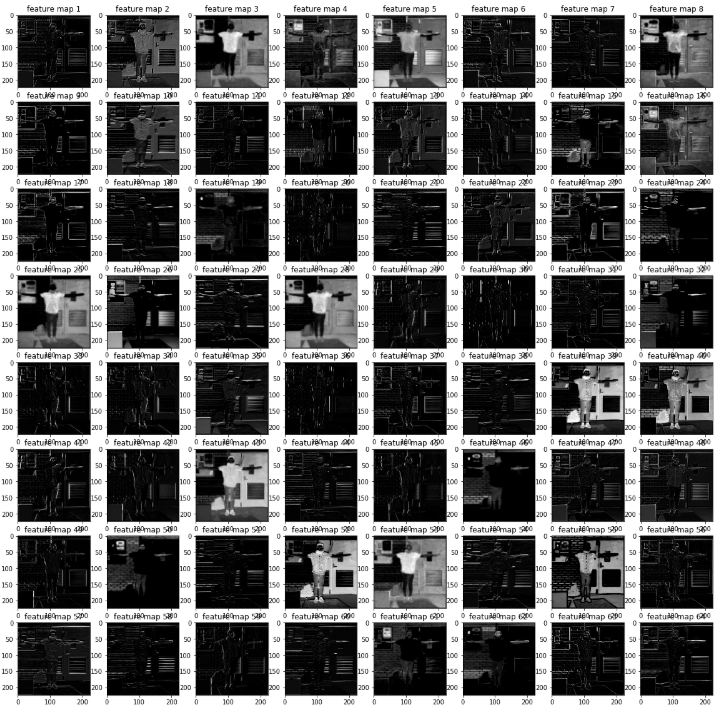
\includegraphics[angle=90,origin=c,width=1\columnwidth]{Figures/convnetFeatureMap.PNG}
\decoRule
\caption[Visualizing of all the feature map of the convolutional layer.]{ Visualizing of all the feature map of the convolutional layer..}
\label{fig:accuracycomparison2}
\end{figure}


\begin{figure}[ht]
\centering
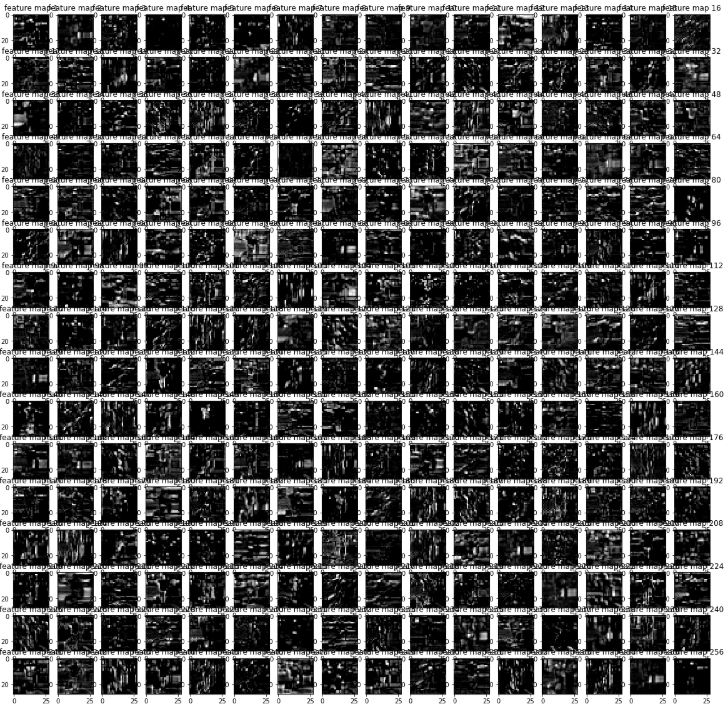
\includegraphics[angle=90,origin=c,width=1\columnwidth]{Figures/maxpoolingFeaturemap.PNG}
\decoRule
\caption[Visualizing of all the feature map of the max pooling layer.]{ Visualizing of all the feature map of the max pooling layer.}
\label{fig:accuracycomparison2}
\end{figure}



\lstinputlisting[
	caption= Script to split the dataset to train, test, validation, % Caption above the listing
	label=lst:luftballons, % Label for referencing this listing
	language=Python, % Use Perl functions/syntax highlighting
	frame=single, % Frame around the code listing
	showstringspaces=false, % Don't put marks in string spaces
	numbers=left, % Line numbers on left
	numberstyle=\tiny, % Line numbers styling
	]{Chapters/code/appendices3.py}
	

\lstinputlisting[
	caption= Script to load a video from the dataset, % Caption above the listing
	label=lst:luftballons, % Label for referencing this listing
	language=Python, % Use Perl functions/syntax highlighting
	frame=single, % Frame around the code listing
	showstringspaces=false, % Don't put marks in string spaces
	numbers=left, % Line numbers on left
	numberstyle=\tiny, % Line numbers styling
	]{Chapters/code/appendices4.py}
	
\lstinputlisting[
	caption= Script to show the data preprocessing pipeline, % Caption above the listing
	label=lst:luftballons, % Label for referencing this listing
	language=Python, % Use Perl functions/syntax highlighting
	frame=single, % Frame around the code listing
	showstringspaces=false, % Don't put marks in string spaces
	numbers=left, % Line numbers on left
	numberstyle=\tiny, % Line numbers styling
	]{Chapters/code/appendices5.py}
% Please add the following required packages to your document preamble:
% \usepackage[table,xcdraw]{xcolor}
% If you use beamer only pass "xcolor=table" option, i.e. \documentclass[xcolor=table]{beamer}
% \usepackage{lscape}
% \usepackage{longtable}
% Note: It may be necessary to compile the document several times to get a multi-page table to line up properly
